
%%%%%%%%%%%%%%%%%%%%%%%%%%%%%%%%%%%%%%%%%%%%%%%%%%%%%%%%%%%%%%%%%%%%%%%%%
%           Capítulo 3: Mapeo de Henon
%%%%%%%%%%%%%%%%%%%%%%%%%%%%%%%%%%%%%%%%%%%%%%%%%%%%%%%%%%%%%%%%%%%%%%%%%
\chapter{Ejemplos de aplicación del método}
\label{SeccionEstandar}\section{Mapeo Estándar}
En el capítulo anterior ya mostramos cómo se aplica el método de manera algebráica para el caso de este mapeo. Utilizando el método ya programado se hicieron diferentes cálculos para comparar con los resultados presentados en \citep{Mireles}. Una de las razones de estudiar el mapeo estándar, además de usarlo como una forma de validación, es porque del mapeo conocemos muchas cosas. Por otro lado queremos mostrar lo importante que es tener una parametrización analítica. Aunque el estudio cualitativo del mapeo puede darnos información útil, tener una parametrización de las variedades relacionadas a sus puntos fijos convierte el análisis en algo cuantitativo y semianalítico. El objetivo de esta sección es mostrar algunas de las cosas que son posibles alcanzar en términos de este análisis, además de la forma en la que se usa el método desde Julia.\\

En el mapeo estándar \eqref{mapeo estandar} uno de los puntos fijos es el origen de coordenadas $\mathbf{x}_{1}=(0,0)$. Utilizando el método programado se calcularon las variedades estables e inestables para diferentes valores del parámetro en el mapeo. El objetivo de hacer éstas fue reproducir los resultados de J.D. Mireles que presenta en sus notas \cite{Mireles}. En tales notas no aparece el orden del polinomio ni el error específico, sin embargo se intentó reproducir al menos gráficamente los resultados. Dependiendo del orden del polinomio que se calcule y del parámetro del mapeo se podrá llegar más lejos del punto fijo.  
\begin{figure}[H]
 \centering
 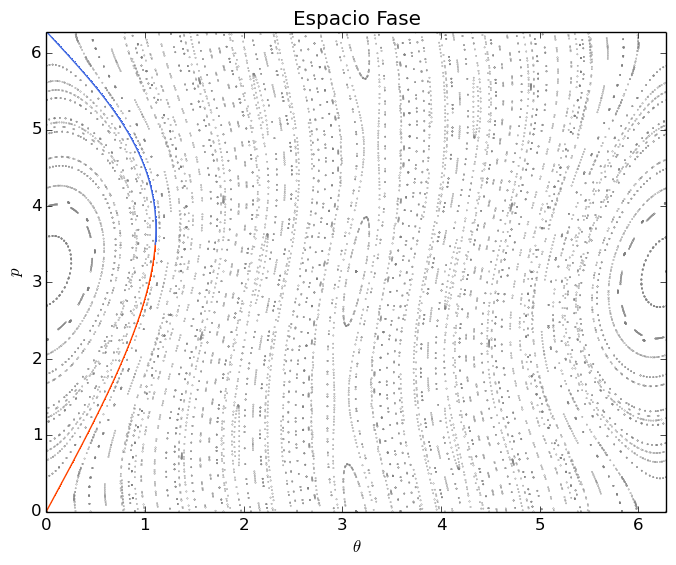
\includegraphics[scale=0.6]{estandark03}
 \caption{\footnotesize $W^{s},W^{u}$ de oden $25$ en el mapeo estándar con $\kappa=0.3$ y $t_{max}=3.0$.}
 \label{estandar03}
\end{figure}

\begin{figure}[H]
\centering
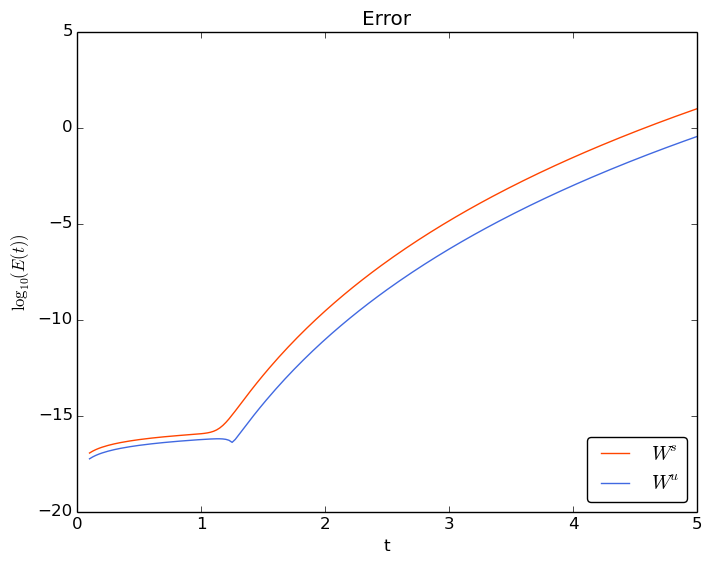
\includegraphics[scale=0.6]{error_est_k03} 
\caption{Error en las variedades de la figura \ref{estandar03}.}
\label{error est k03}
\end{figure}


\begin{figure}[H]
\centering
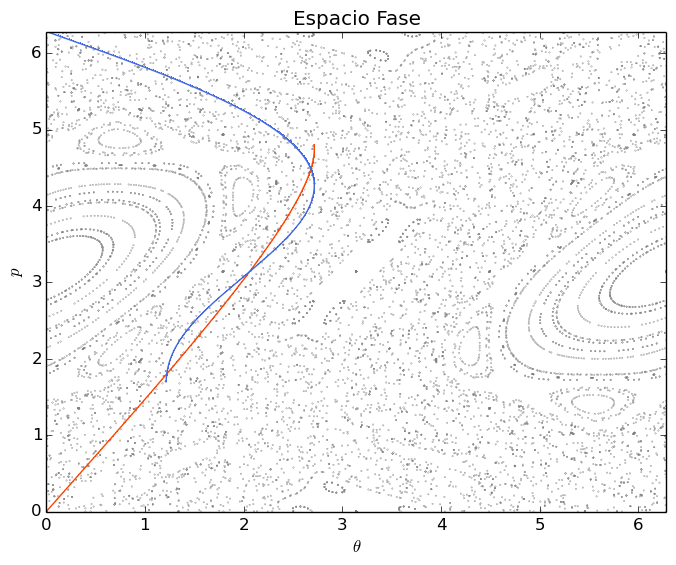
\includegraphics[scale=0.6]{estandark15}
\caption{$W^{s},W^{u}$ de orden $80$ en el mapeo estándar con $\kappa=1.5$ y $t_{max}=13.0$.}
\label{estandar15}
\end{figure}

\begin{figure}[H]
\centering
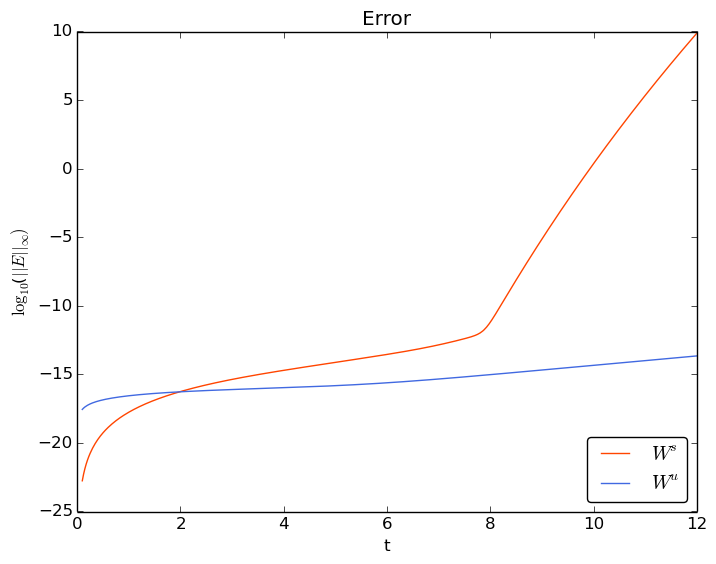
\includegraphics[scale=0.6]{error_est_k15} 
\caption{Error en las variedades de la figura \ref{estandar15}.}
\label{error est k15}
\end{figure}




\begin{figure}[H]
\centering
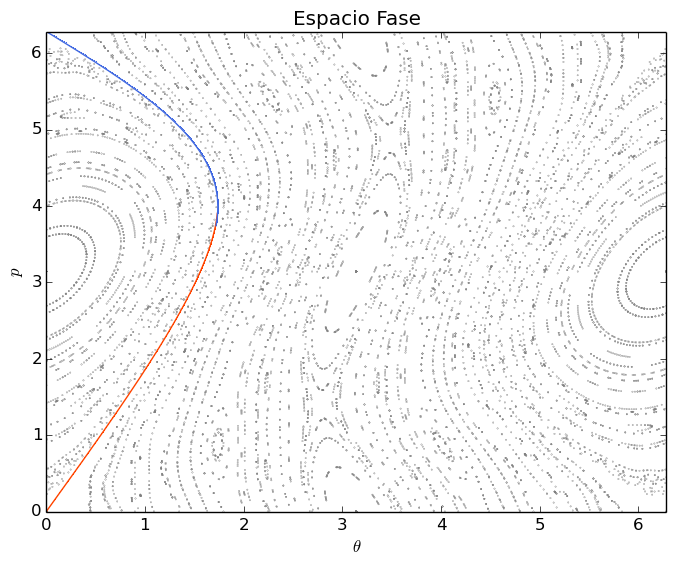
\includegraphics[scale=0.6]{estandark07}
\caption{$W^{s},W^{u}$ de orden 70 en el mapeo estándar con $\kappa=0.7$ y $t_{max}=5.5$.}
\label{estandar07}
\end{figure}

\begin{figure}[H]
\centering
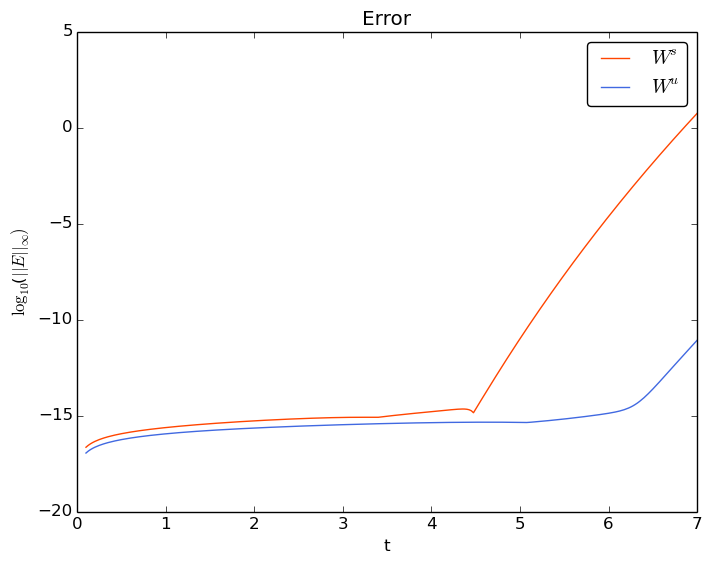
\includegraphics[scale=0.6]{error_est_k07} 
\caption{Error en las variedades de la figura \ref{estandar07}.}
\label{error est k07}
\end{figure}


En las figuras \ref{estandar03}-\ref{error est k07} se muestran los resultados de la parametrización de las variedades estable e inestable asociadas al punto fijo $\mathbf{x}_{1}$ para diferentes valores del parámetro $\kappa$, junto con cada una aparece su respectiva gráfica del error numérico.   Los cálculos se hicieron utilizando números de punto flotante de 64 bits(Float64). Para las figuras \ref{estandar03}, \ref{estandar07} se puede ver que las variedades se juntan de manera que parecen ser tangentes, mientras que para el caso de la figura \ref{estandar15} observamos varias intersecciones entre las variedades. En todos los casos el error se comporta de manera similar, manteniéndose prácticamente constante hasta cierto valor del parámetro $t$ y creciendo de forma exponencial después del mismo. La curva será entonces confiable hasta valores del parámetro que no excedan el punto donde el error crece rápidamente.  \\


Para observar como cambiaba el comportamiento del error respecto del orden de la parametrización se calcularon polinomios de diferente orden que parametrizan a la variedad inestable del mapeo con $\kappa=0.3$, el resultado se muestra en la figura \ref{erroresf64}. Observamos que mientras más grande sea el orden del polinomio mejor es la aproximación, pues podemos llegar a valores del parámetro más grandes, que se traduce en ir más lejos en la variedad inestable. \\

\begin{figure}[H]
\centering
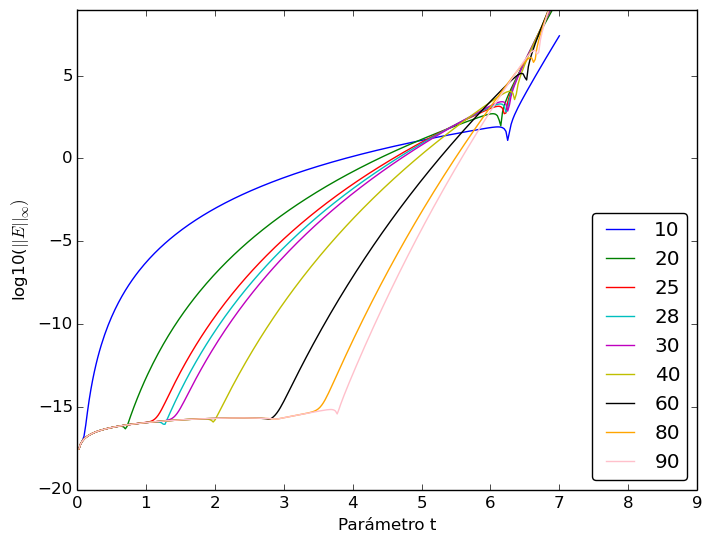
\includegraphics[scale=0.6]{error_estandar_orden}
\caption{Curvas de error para diferentes órdenes en el mapeo estándar, $\kappa=0.3$. }
\label{erroresf64}
\end{figure}
A fin de mostrar que el error es de alguna manera controlable se usaron números de precisión extendida para hacer cálculos análogos a los anteriores. En la figura \ref{erroresBig} se muestran los resultados para parametrizaciones de ordenes entre $10$ y $80$. Observamos un comportamiento análogo, de tal manera que para cada orden diferente de parametrización hay un valor diferente del parámetro en el cual pasa de un error que no crece significativamente a un error que crece de manera abrupta. También notamos que al usar precisión extendida el error cerca del punto fijo es imperceptible pero en la parte donde crece, tiene un crecimiento más pronunciado que en el caso de números de punto flotante. 

\begin{figure}[H]
\centering
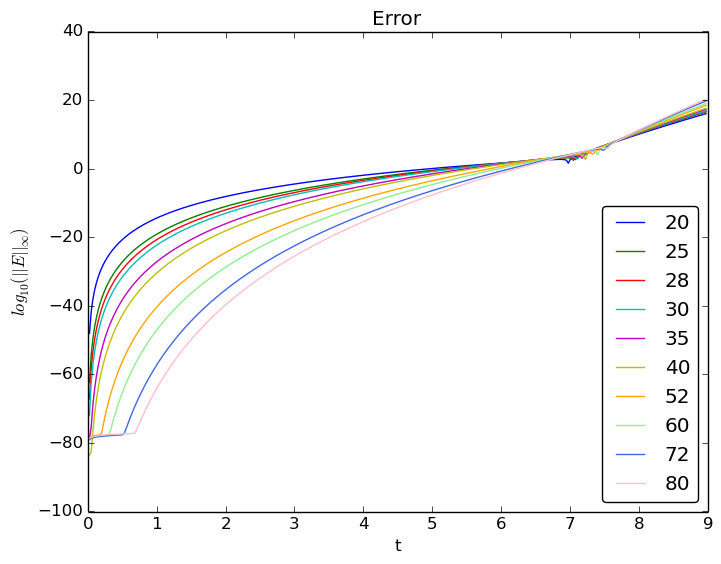
\includegraphics[scale=0.6]{error_estandar_orden_big}
\caption{Curvas de error para diferentes órdenes usando precisión extendida ,$\kappa=0.3$. }
\label{erroresBig}
\end{figure}

Como ya mencionamos antes la variedad inestable del mapeo inverso corresponde a la variedad estable del mapeo, si se usa el mismo método calculando la variedad inestable del mapeo inverso \eqref{mapeo estandar inverso} podemos controlar mejor el error numérico. Para mostrar esto hicimos una comparación parametrizando la variedad estable mediante el mapeo inverso y el mapeo inicial. Los polinomios fueron del mismo orden y lo que se observó en el error se muestra en la figura \ref{erroresinverso}.


\begin{figure}[H]
\centering
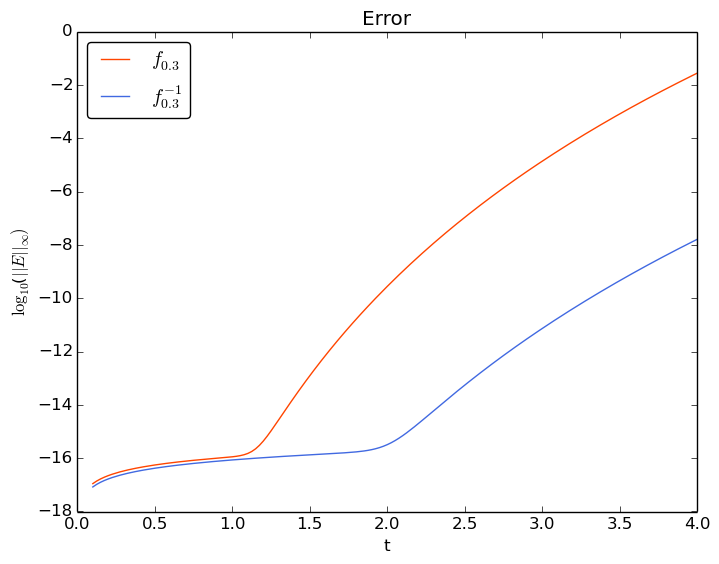
\includegraphics[scale=0.6]{mapeoinver}
\caption{Error para las parametrizaciones usando el mapeo y el mapeo inverso con polinomios de orden $20$ y $\kappa=0.3$. }
\label{erroresinverso}
\end{figure}

Usar el mapeo inverso para calcular la variedad estable resulta ser mejor que usar el mapeo normal. El error se mantiene casi sin cambios hasta una valor de $t$ mayor en el caso del mapeo inverso. 




\label{henon-seccion}\section{Mapeo de Hénon}
El mapeo de Hénon se define como \cite{devaney}
\begin{eqnarray}
\mathbf{f}_{a,b}(x,y)=\left( \begin{array}{lcc}
             a-by-x^{2}\\
             \\ x
             \end{array}
             \right), \label{Henon}
\end{eqnarray}

siendo el mapeo inverso
\begin{eqnarray}
\mathbf{f}^{-1}_{a,b}(x,y)=\left( \begin{array}{lcc}
             y\\
             \\ (x+y^{2}-a)/-b
             \end{array}
             \right). \label{HenonI}
\end{eqnarray} 

       
Para poder analizarlo debemos linearizar el sistema. Primero obtenemos el jacobiano 
            
\begin{eqnarray}
D\mathbf{f}_{a,b}(x,y)= \left( \begin{array}{lcc}
                -2x & -b\\
                \\ 1 & 0
                \end{array}
                \right).
\end{eqnarray}

                
Notamos que el determinante del jacobiano no es igual a uno sino $\det(D\mathbf{f}_{a,b}(x,y))=b$.
El determinante es constante, entonces será Hamiltoniano en el caso en que $b$ sea igual a uno o menos uno. Analizaremos estos casos, encontrando los puntos fijos
\begin{eqnarray}
\mathbf{f}_{a,b}(x,y)=\left( \begin{array}{lcc}
               a-by-x^{2}\\
               \\ x
               \end{array}
               \right) = \left(\begin{array}{lc}
               x \\
               \\ y
               \end{array}
               \right),
\end{eqnarray}
              
lo que implica que $a-by-x^{2}=x$ y $x=y$ de donde es claro que la primer ecuación queda
\begin{eqnarray*}
x^{2}+(b+1)x-a=0, 
\end{eqnarray*}
que se puede resolver usando la fórmula general
\begin{eqnarray*}
x=\frac{-(b+1)\pm ((b+1)^{2}+4a)^{1/2} }{2},
\end{eqnarray*}
para el caso en que $b=1$ se tiene
\begin{eqnarray}
x=\frac{-2\pm 2(1+a)^{1/2} }{2}.
\end{eqnarray}
Al escoger $b=1$ garantizamos estar en un sistema Hamiltoniano, mientras que $a$ debe escogerse de manera que resulten puntos fijos hiperbólicos. La figura \ref{Henon1} muestra un ejemplo en cálculos de variedades para el mapeo de Hénon, junto con el error. 
\begin{figure}[H]
\centering
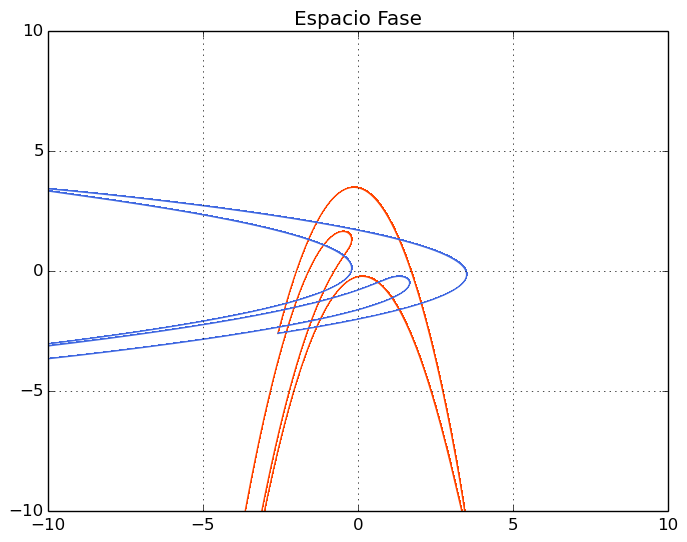
\includegraphics[scale=0.6]{henon1}
\caption{$W^{u}$ y $W^{s}$ de orden 45 con $t_{max}=1000.0$ para el mapeo de Hénon con $a=1.5$,$b=1$.}
\label{Henon1}
\end{figure}

\begin{figure}[H]
\centering
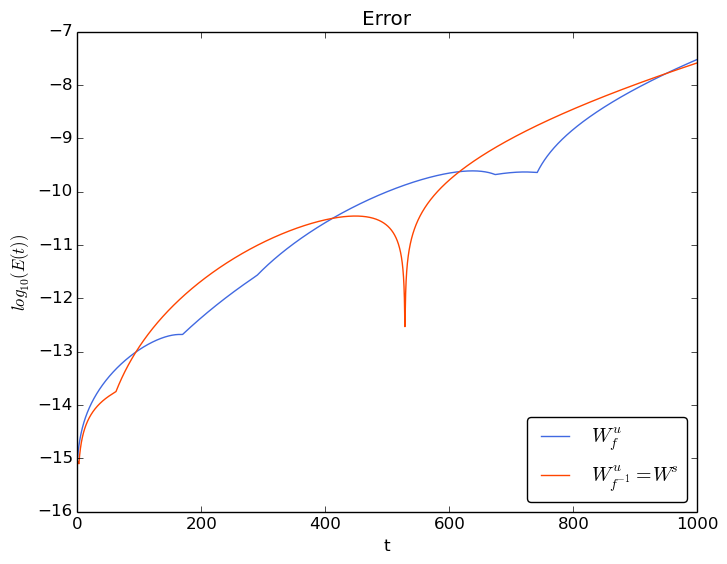
\includegraphics[scale=0.6]{ErrorHenon1}
\caption{Error asociado a las variedades de la figura \ref{Henon1}.}
\label{ErrorHenon1}
\end{figure}
Las variedades que aparecen en la figura \ref{Henon1} fueron calculadas con el mapeo de Hénon inicial \eqref{Henon}, las variedades se observan simétricas, aún así las parametrizaciones son diferentes. Puede verse en el error, figura \ref{ErrorHenon1}, que la variedad estable tiene un mayor error que la variedad inestable, mientras en la inestable el error cambia cinco órdenes de magnitud, en todo el intervalo del parámetro, el error de la variedad estable cambia en al menos quince órdenes de magnitud. \\

A diferencia del mapeo estándar en éste mapeo las órbitas pueden irse al infinito, es decir no están  constreñidas en una sección fija, lo que representa un mayor reto en cuanto a la parametrización ya que el polinomio debe ser tal que pueda regresar varias veces. De hecho podemos observar que se necesitan valores realmente grandes, comparados con los del mapeo estándar, para observar los cruces de las variedades. También esta situación hace que el error numérico sea mayor que para el estándar. \\

En las figuras \ref{Henon2}, \ref{Henon3} se muestran las variedades calculadas de la misma manera en la que se calcularon para la figura \ref{Henon1}. En \ref{Henon2} las curvas son más cerradas y se necesita de un polinomio de orden mayor que en el caso de \ref{Henon3} para observar los cortes. 
\begin{figure}[H]
\centering
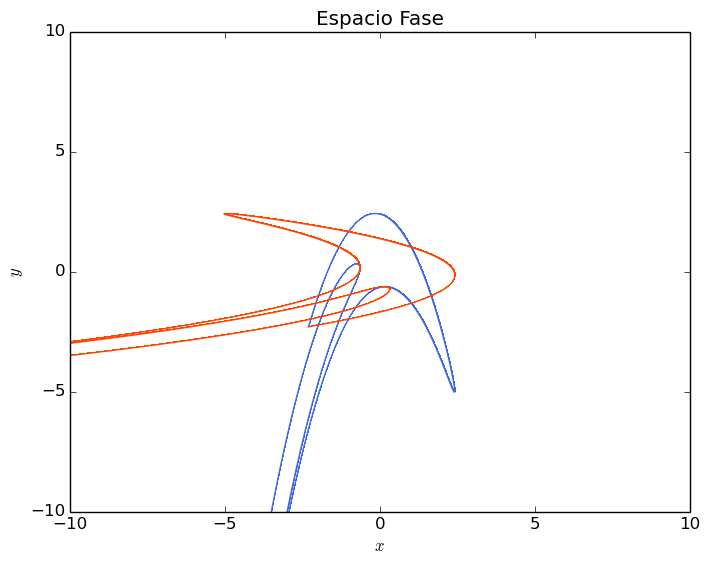
\includegraphics[scale=0.6]{henon2}
\caption{$W^{u}$, $W^{s}$ de orden $50$ y $t_{max}=800.0$ para el mapeo de Hénon con $a=0.7$,$b=1.$.}
\label{Henon2}
\end{figure}

\begin{figure}[H]
\centering
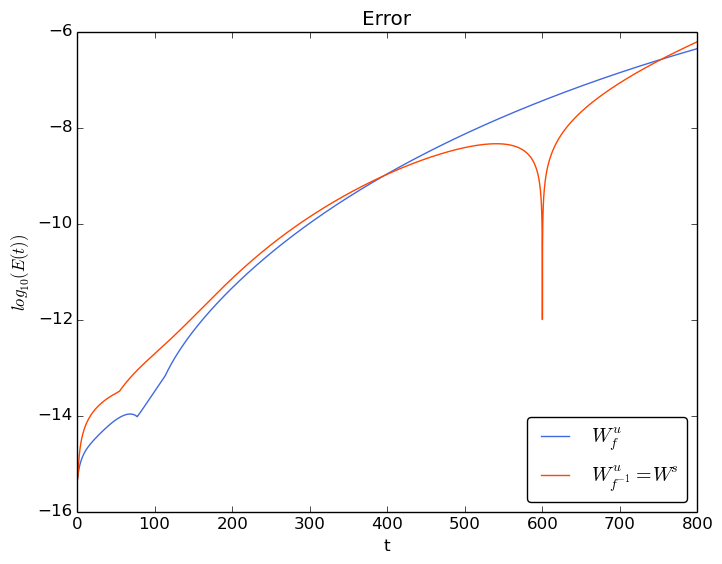
\includegraphics[scale=0.6]{ErrorHenon2}
\caption{Error asociado a las variedades de la figura \ref{Henon2}.}
\label{Henon2}
\end{figure}


\begin{figure}[H]
\centering
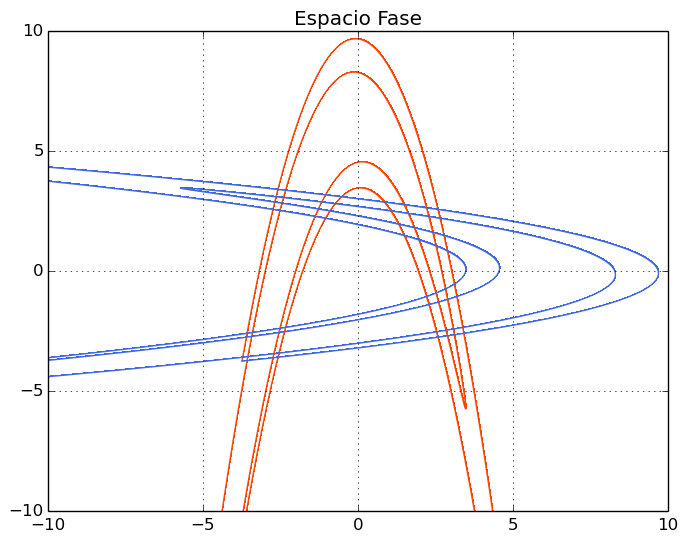
\includegraphics[scale=0.6]{henon3}
\caption{$W^{u}$, $W^{s}$ de orden $78$ y $t_{max}=4000.0$ para el mapeo de Hénon con $a=6.5$,$b=1.$.}
\label{Henon3}
\end{figure}

\begin{figure}[H]
\centering
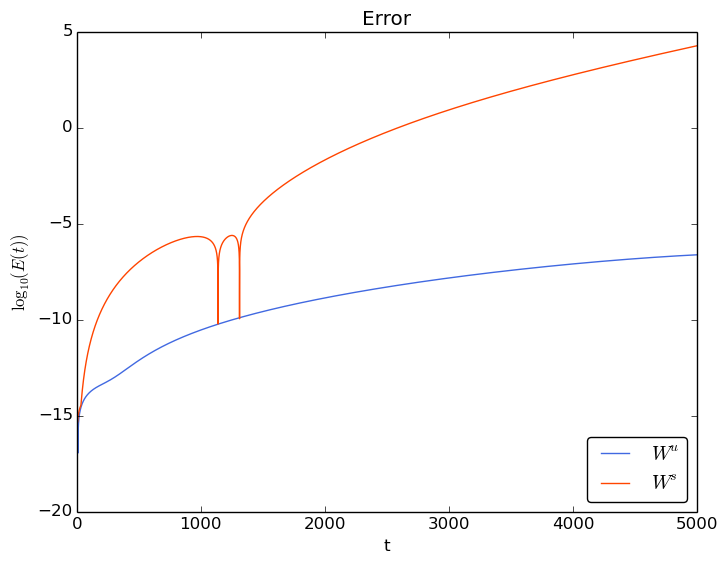
\includegraphics[scale=0.6]{ErrorHenon3}
\caption{Error asociado a las variedades de la figura \ref{Henon3}.}
\label{Henon3}
\end{figure}


Así que con el orden suficiente es posible observar los cruces de ambas variedades, retomaremos esto en la última sección. 

\label{jung-seccion}\section{Mapeo exponencial}
El último mapeo que se estudió fue uno presentado en el artículo \citep{Jung} el cual queda definido por 
\begin{eqnarray}
\mathbf{j}_{a}(x,y)=\left(\begin{array}{lcc}
             x+y\\
             \\ y+af(x+y)
             \end{array}\right),
\label{Jung}
\end{eqnarray}

que describe el movimiento de una partícula pateada, donde la coordenada $x$ representa la posición en una dimensión mientras que la coordenada $y$ es el momento, $a$ es un parámetro libre. La función $f$ es la responsable de describir la fuerza aplicada, en el artículo \cite{Jung} se escoge
\begin{eqnarray*}
f(x)=x(x-1)e^{-x}.
\end{eqnarray*}
A este mapeo le corresponde su mapeo inverso
\begin{eqnarray}
\mathbf{j}^{-1}_{a}(x,y)=\left(\begin{array}{lcc}
             x-y+ax(x-1)e^{-x}\\
             \\ y-ax(x-1)e^{-x}
             \end{array}\right).
             \label{jungI}
\end{eqnarray}
Los puntos fijos encontrados del sistema son $\mathbf{x}_{0}=(1,0), \mathbf{x}_{1}=(0,0)$ donde $\mathbf{x}_{0}$ es un punto fijo hiperbólico. El punto $\mathbf{x}_{1}$ es un punto elíptico mientras el valor del parámetro $a$ sea menor a 4, para valores de $a \geq 4$ se torna inverso hiperbólico.\\

Aplicando el mismo mecanismo que en los casos pasados se obtuvieron las figuras \ref{jung1}-\ref{errorjung2} que muestran cómo se comportan las variedades aún en el caso en que el sistema no sea completamente hiperbólico. Como en los casos anteriores el error asociado a la variedad estable es mayor que el asociado a la inestable. El orden al que se debe llegar en los polinomios para observar algunos de los cortes de las variedades es más alto en comparación con el mapeo de Hénon debido a que en este caso se esta aproximando una función exponencial.

\begin{figure}[H]
\centering
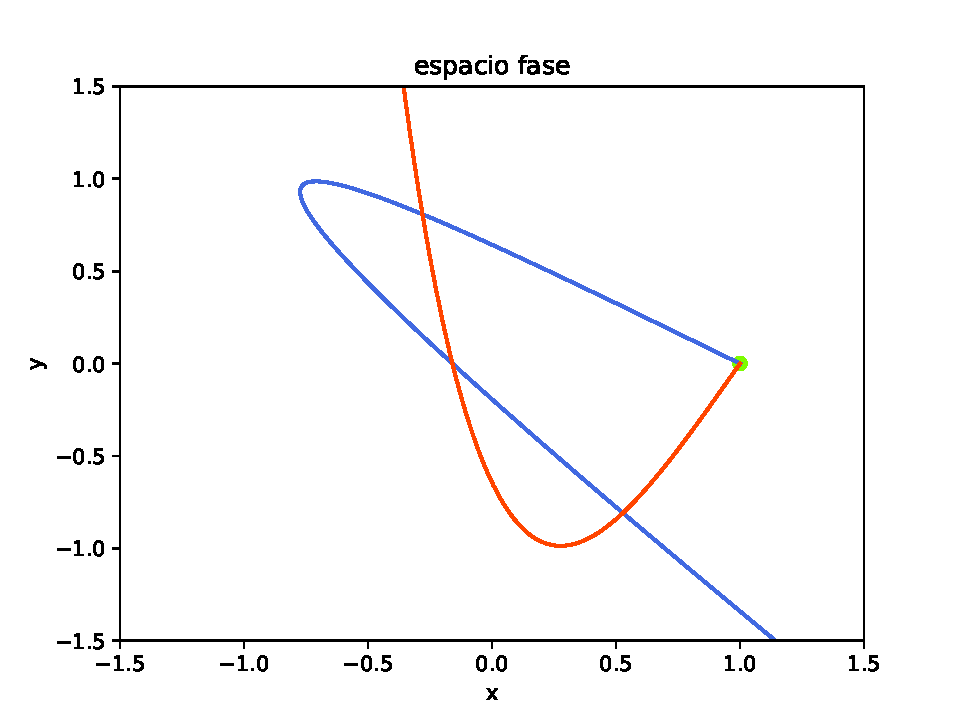
\includegraphics[scale=0.6]{jung34}
\caption{$W^{s}$ de orden 93, $W^{u}$ de orden 86 con $t_{max}=5.5$, con $a=3.4$ en el punto fijo $x_{0}$.}
\label{jung1}
\end{figure}


\begin{figure}[H]
\centering
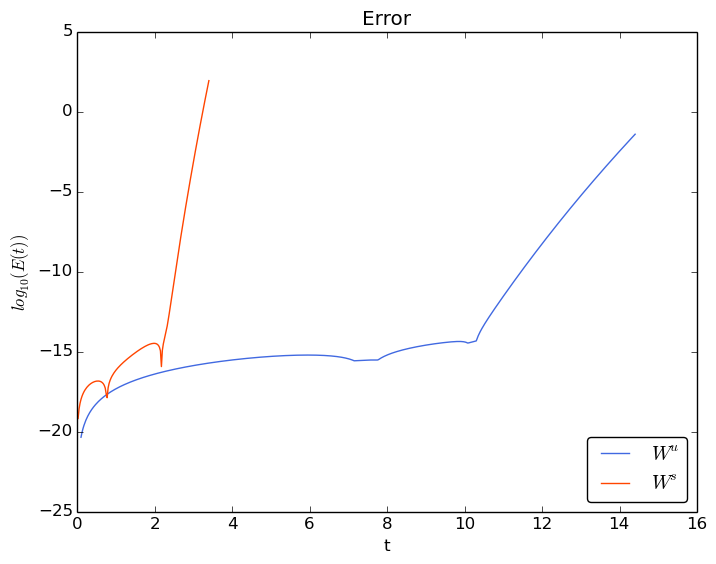
\includegraphics[scale=0.6]{error_jung34}
\caption{Error asociado a las variedades de la figura \ref{jung1}.}
\label{errorjung1}
\end{figure}




\begin{figure}[H]
\centering
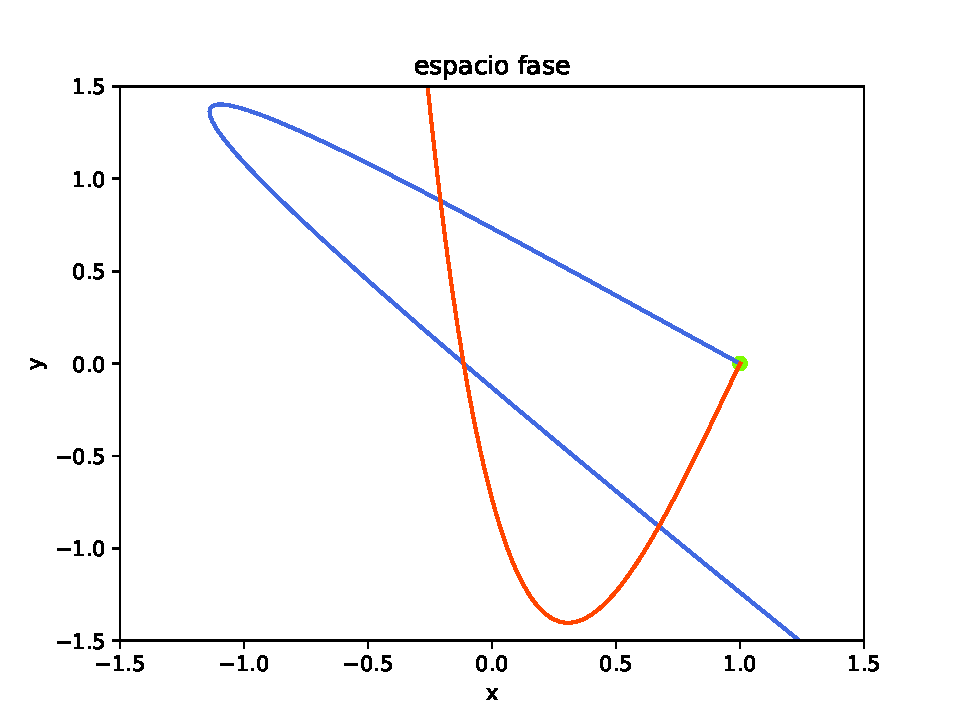
\includegraphics[scale=0.6]{jung57}
\caption{$W^{s}$ de orden 93, $W^{u}$ de orden 86 con $t_{max}=6.5$, con $a=5.7$ en el punto fijo $x_{0}$.}
\label{jung2}
\end{figure}


\begin{figure}[H]
\centering
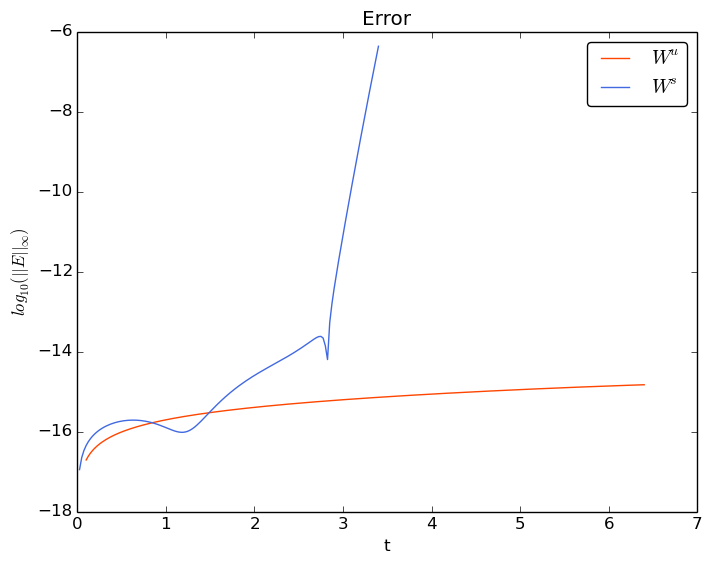
\includegraphics[scale=0.6]{error_jung57}
\caption{Error asociado las variedades de la figura \ref{jung2}.}
\label{errorjung2}
\end{figure}
Se puede observar en las figuras \ref{errorjung1}, \ref{errorjung2} que en la variedad estable el error crece de manera abrupta antes que el error de la variedad inestable. Ambas curvas del error tienen la misma forma, pero es claro que no se puede llegar tan lejos en la variedad estable. El mapeo es más sensible que los dos mapeos pasados, algunos órdenes resultaban no ajustarse a la variedad más allá de valores del parámetro menor a uno. 


\section{Convergencia}
Además de medir el error asociado a la parametrización consideramos importante tomar en cuenta la convergencia de los coeficientes de los polinomios. En casos como el mapeo exponencial en que las variedades se acercan a puntos fijos de diferente naturaleza puede ocurrir que tal cercanía afecte la forma de parametrización. Para ello se implementaron dos formas de revisar la convergencia, la de Hadamard \eqref{hadamard} y la de tres términos \eqref{tres terminos}. \\

La figura \ref{convergenciaEst15} muestra la convergencia de los polinomios de orden 25 que parametrizan la variable $\theta$ en el mapeo estándar para las variedades estable e inestable con $\kappa=1.5$ a la que corresponde el espacio fase mostrado en \ref{estandar15}. En el caso de la variedad estable se ve que los coeficientes cambian de manera abrupta al principio pero después de cierta $n$ el cociente es casi cero. Para el caso de la variedad inestable los coeficientes cambian de manera suave y el cociente también se acerca a cero. En ambos casos podemos decir que los coeficientes de la parametrización convergen a cero.  
\begin{figure}[H]
\centering
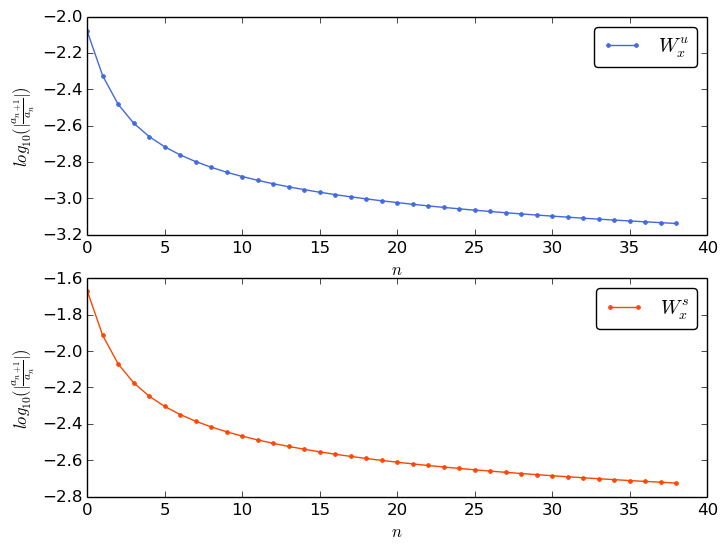
\includegraphics[scale=0.5]{converEst15}
\caption{Convergencia de Hadamard asociada a los polinomios para $\theta$ en las variedades del mapeo estándar con $\kappa=1.5$.}
\label{convergenciaEst15}
\end{figure}

La figura \ref{convergenciaHenon1} muestra la convergencia de las parametrizaciones de orden 45 para la variable $x$ en el mapeo de Hénon con $a=1.5$. En ambos casos la convergencia parece suave y tiende a cero igual que en el caso del mapeo estándar.

\begin{figure}[H]
\centering
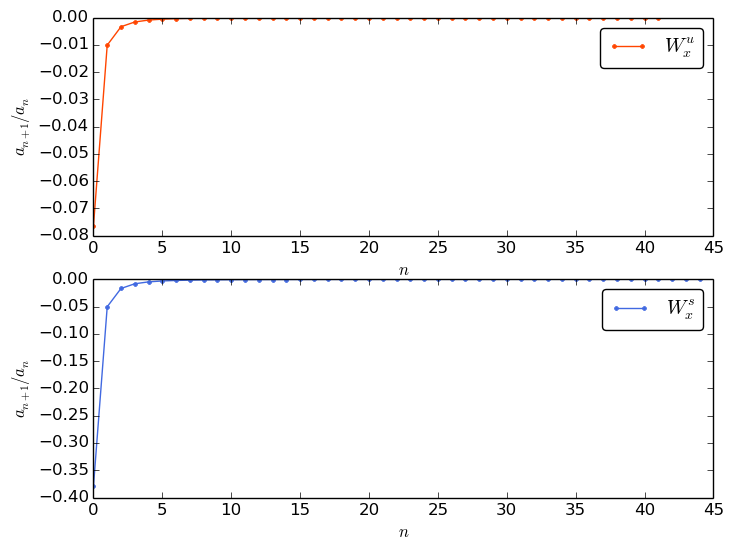
\includegraphics[scale=0.5]{converHenon1}
\caption{Convergencia de Hadamard asociada a los polinomios para $x$ en las variedades del mapeo de Hénon con $a=1.5$.}
\label{convergenciaHenon1}
\end{figure}


Para el mapeo exponencial realizamos los dos criterios de convergencia. La figura \ref{convergenciaJH} muestra el criterio de Hadamard \eqref{hadamard}, para los polinomios que parametrizan la variable x en cada variedad, se ve que hay una convergencia clara de los coeficientes. Lo mismo ocurre en la figura \ref{convergenciaJ3} en dónde se usó el criterio de tres términos, \eqref{tres terminos}.

\begin{figure}[H]
\centering
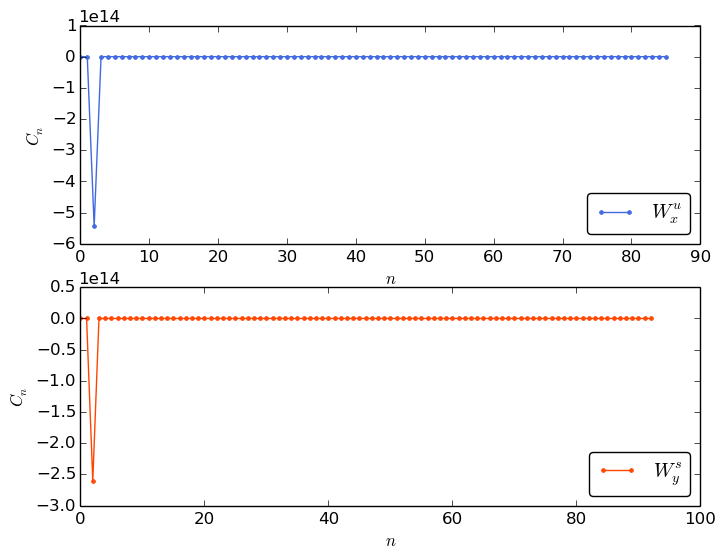
\includegraphics[scale=0.5]{convergenciaJungH57}
\caption{Convergencia de Hadamard asociada a las variedades mostradas en la figura \ref{jung2}.}
\label{convergenciaJH}
\end{figure}


\begin{figure}[H]
\centering
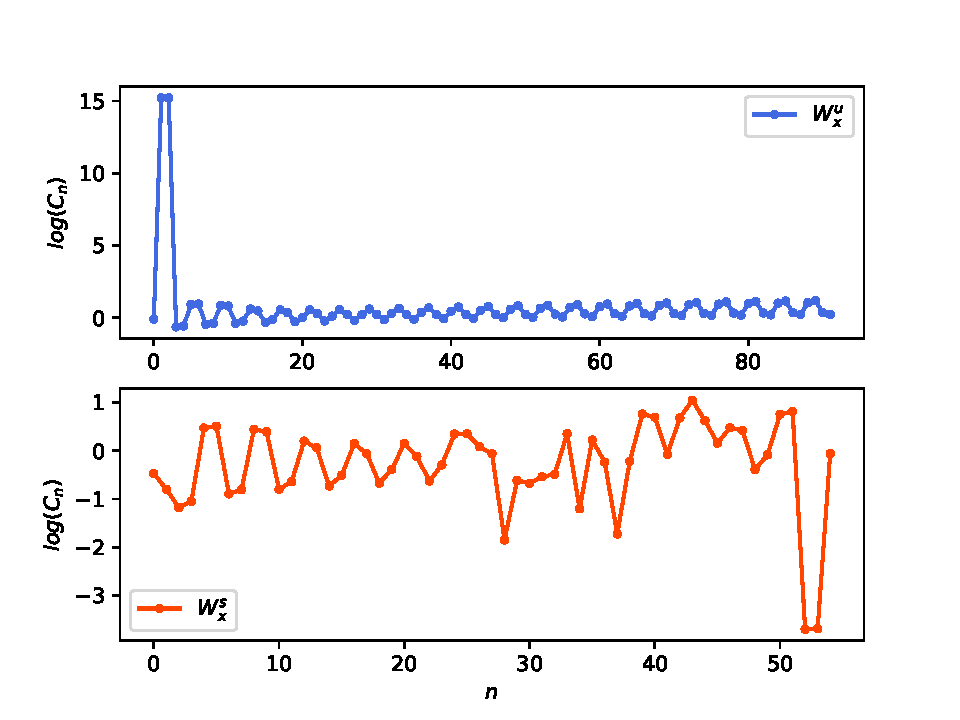
\includegraphics[scale=0.5]{convergenciaJungT57}
\caption{Convergencia de tres términos asociada a las variedades en la figura \ref{jung2}.}
\label{convergenciaJ3}
\end{figure}

Estudiar la convergencia de las parametrizaciones puede dar una idea de cómo se va modificando el polinomio si se cambia el orden, en mapeos más sensibles puede ser determinante para saber a qué orden es conveniente aproximar. 

\section{Existencia de puntos homoclínicos/heteroclínicos}

Siendo que el resultado son polinomios se puede aplicar el método de Newton en dos dimensiones o cualquier otro para resolver $P^{u}=P^{s}$ y encontrar puntos homoclínicos o heteroclínicos. Por suerte existe una paquetería en Julia que hace cálculos numéricos validados \texttt{ValidatedNumerics}\cite{validated} dentro de la cuál se tiene un paquete para aritmética de intervalos \texttt{IntervalArithmetic}\citep{interval} y para encontrar raíces \texttt{IntervalRootFinding}\cite{root} además del paquete \texttt{Static Arrays}\cite{static} que permite manipular intervalos.\\ 

El paquete \cite{validated} hace cálculos de computación rigurosa con números de punto flotante usando el paquete de aritmética de intervalos, que efectúa operaciones con intervalos en lugar de números. Mientras que \cite{root} automatiza el métodos populares como el de Newton para encontrar raíces de funciones, en este caso se garantiza que la respuesta correcta se encuentra en un intervalo. Para entender mejor cómo funcionan cada una de las paqueterías así como la teoría rigurosa detrás de éstos recomendamos revisar las lecturas \cite{ramon},\cite{Numerics}. De manera breve podemos decir que los paquetes ya mencionados generalizan las operaciones y funciones ahora en términos de conjuntos, de tal manera que que la solución contenga la respuesta correcta. \\

Las variedades parametrizadas que resultan del método son polinomios, por lo que con las paqueterías  mencionadas se puede analizar cuando dos de ellas se cruzan. Concretamente se tienen  $W^{s}(t)=(P_{x}(t),P_{y}(t))$ y $W^{u}(\tau)=(P_{x}(\tau),P_{y}(\tau))$ de órdenes no necesariamente iguales, y lo que se busca es:
\begin{eqnarray}
W^{s}(t)=W^{u}(\tau),
\end{eqnarray}
que arrojará como resultado un intervalo $I_{t}$ y otro intervalo $I_{\tau}$, la intersección se encontrará en $I_{t}\times I_{\tau}$. En el espacio fase la intersección se verá como el producto cartesiano de $W^{s}(I_{t})\times W^{u}(I_{\tau})$ formando una sección en la que se garantiza hay un punto homoclínico o heteroclínico. 


\subsection{Estándar}
Usando lo descrito anteriormente se calcularon las intersecciones de las variedades estable e inestable en el mapeo estándar para un valor de $\kappa=1.5$ usando polinomios de orden $120$, además de usar el mapeo inverso \eqref{mapeo estandar inverso} para calcular la variedad estable. Se encontraron cuatro raíces en el intervalo $[-20.,0.]$ para $t$  y $[-15.,0.]$ para $\tau$, con una tolerancia de $10^{-6}$ usando el método de Newton, las cuales son:
\begin{itemize}
\item Root$([-7.16826, -7.16825] \times [-4.45972, -4.45971]$, :unique)
\item Root$([-4.21757, -4.21756] \times [-8.36029, -8.36028]$, :unique)
\item Root$([-2.24983, -2.24982] \times [-14.2093, -14.2092]$, :unique)
\item Root$([-13.4378, -13.4377] \times [-2.62396, -2.62395]$, :unique)
\end{itemize}
El primer intervalo corresponde al parámetro $t$ mientras que el segundo al parámetro $\tau$, la leyenda \texttt{unique} indica que en el intervalo presentado sólo hay una raíz. Las raíces se representan gráficamente en el espacio fase en la figura \ref{cruce_estandar}. 

\begin{figure}[H]
\centering
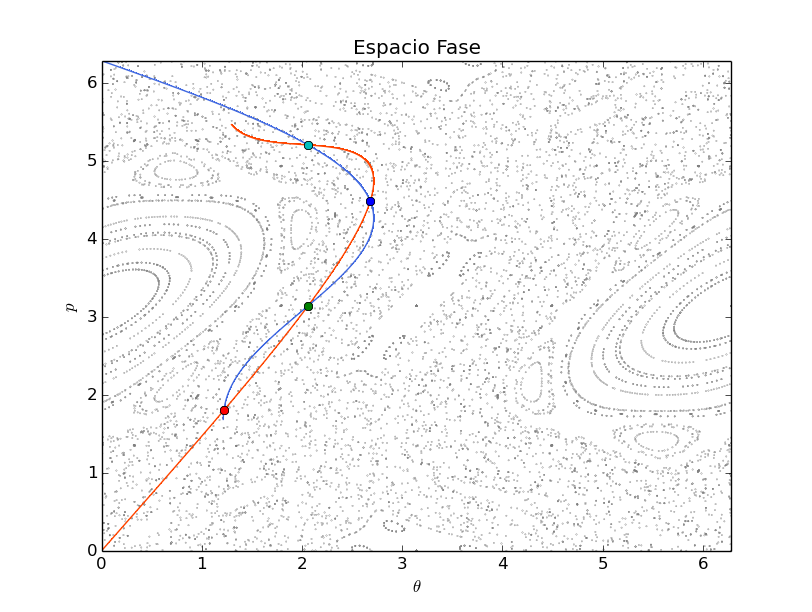
\includegraphics[scale=0.6]{cruce_estandar}
\caption{Cruces de $W^{u},W^{s}$ de orden $120$ para el mapeo estándar con $\kappa=1.5$ .}
\label{cruce_estandar}
\end{figure}
El error asociado al cálculo de las variedades se puede ver en la figura \ref{errorEstCruces}, en dónde se aprecia que los valores aceptables de los parámetros están dentro del intervalo inicial. 

\begin{figure}[H]
\centering
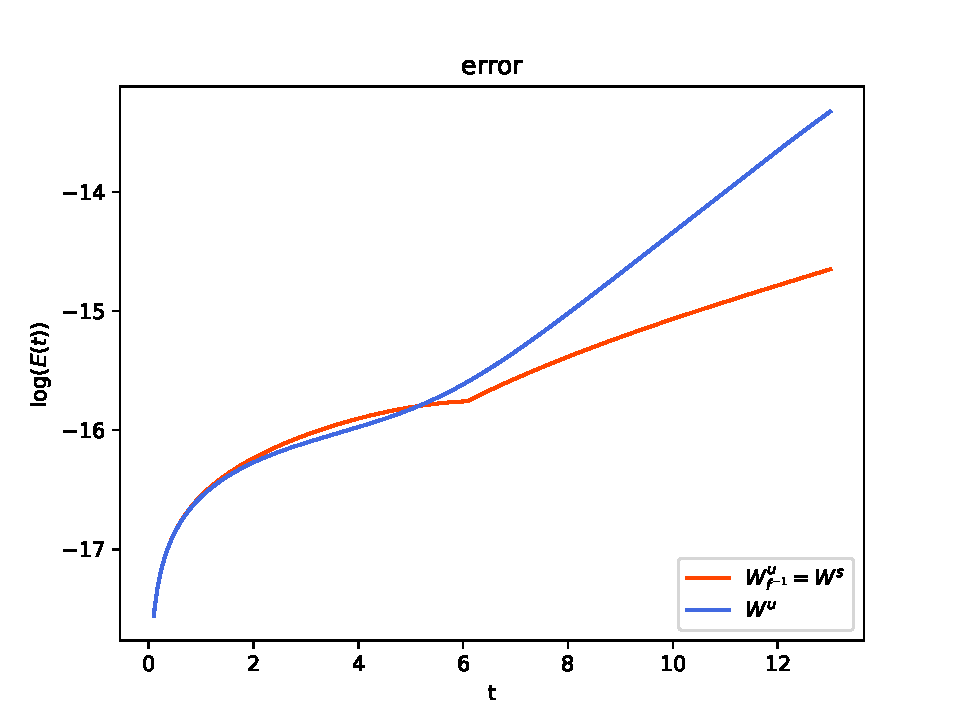
\includegraphics[scale=0.6]{error_cruces_estandar}
\caption{Error en las variedades de la figura \ref{cruce_estandar}.}
\label{errorEstCruces}
\end{figure}

El cálculo numérico riguroso garantiza que la solución está en el intervalo que da como resultado, sin embargo no debemos olvidar que nuestras variedades tienen un error asociado, por lo que es importante quedarse en aquellos intervalos del parámetro donde se tenga un error mínimo. Con las raíces obtenidas podemos asegurar que en el mapeo estándar con el valor del parámetro $\kappa=1.5$ se encuentran cuatro puntos homoclínicos. Si se quiere encontrar más puntos se debe considerar un polinomio de orden mayor o en todo caso usar números de precisión extendida para llegar más lejos en las variedades. 



\subsection{Hénon}
Así como se calcularon las intersecciones en las variedades del mapeo estándar se calcularon ahora para el mapeo de Hénon. En este caso se usó un valor del parámetro $a=1.5$ con un polinomio de orden 45 y el método de Newton con una tolerancia de $10^{-6}$ además de usar el mapeo inverso \eqref{HenonI}, para calcular la variedad estable. Los resultados fueron los siguientes intervalos:
\begin{itemize}
\item[a)] Root$([-1.36597, -1.36596] \times [166.749, 166.75]$, :unique)
\item[b)] Root$([-5.26555, -5.26554] \times [129.577, 129.578]$, :unique)
\item[c)] Root$([-6.77613, -6.77612] \times [33.6142, 33.6143]$, :unique)
\item[d)] Root$([-5.54438e-07, 0] \times [0, 5.54438e-07]$, :unknown)     
\item[e)] Root$([-26.1208, -26.1207] \times [26.1207, 26.1208]$, :unique)  
\item[f)] Root$([-33.6143, -33.6142] \times [6.77612, 6.77613]$, :unique)  
\item[g)] Root$([-129.578, -129.577] \times [5.26554, 5.26555]$, :unique) 
\item[h)] Root$([-166.75, -166.749] \times [1.36596, 1.36597]4$, :unique)
\end{itemize}

La leyenda \texttt{unknown} nos dice que no puede concluir si hay una o más raíces en el intervalo. Si notamos el tercer intervalo contiene al cero $(t,\tau)=(0,0)$ en el cual se cortan las variedades pues representa el punto fijo. La figura \ref{crucesH} representa con un punto los cortes encontrados en las variedades.
\begin{figure}[H]
\centering
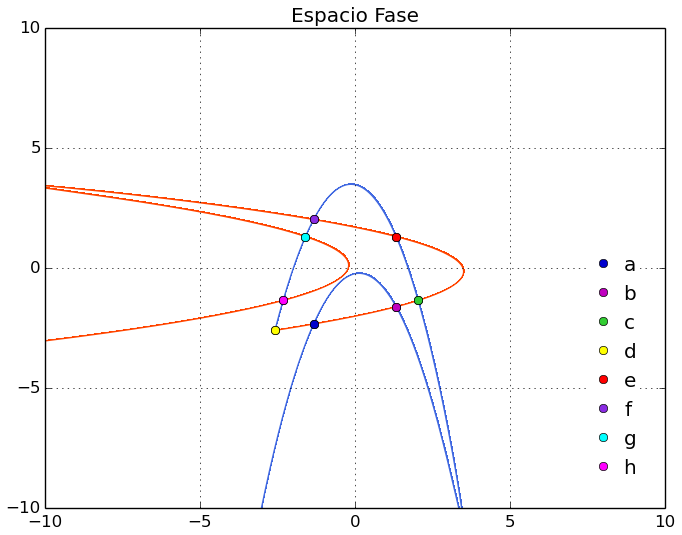
\includegraphics[scale=0.5]{crucesL}
\caption{Cruces de $W^{u},W^{s}$ encontrados en el intervalo $[-400.,0.] \times [0.,400.]$ .}
\label{crucesH}
\end{figure}
Los puntos de color son sólo para indicar cuales intersecciones fueron encontradas. Para los intervalos encontrados se hizo una gráfica que representa la región en el espacio fase donde se encuentra el cruce, las figuras \ref{cruce1H}-\ref{cruce8H} muestran cada una de ellas.

\begin{figure}[H]
\centering
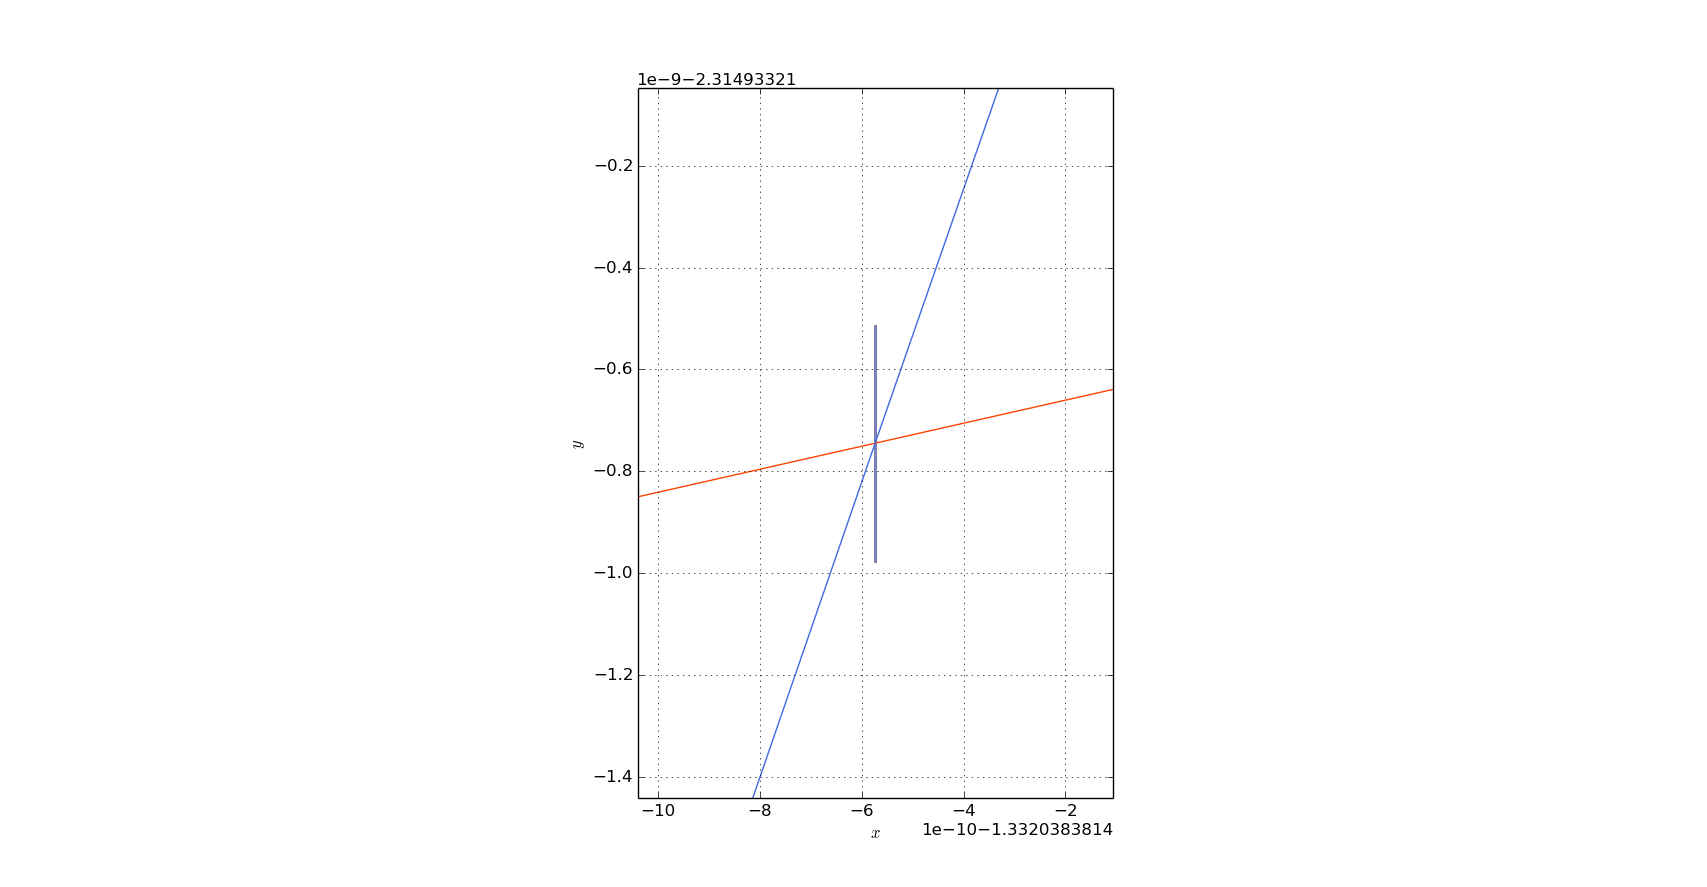
\includegraphics[scale=0.4]{cruce1}
\caption{Cruce de $W^{u},W^{s}$ encontrado con el intervalo a.}
\label{cruce1H}
\end{figure}

\begin{figure}[H]
\centering
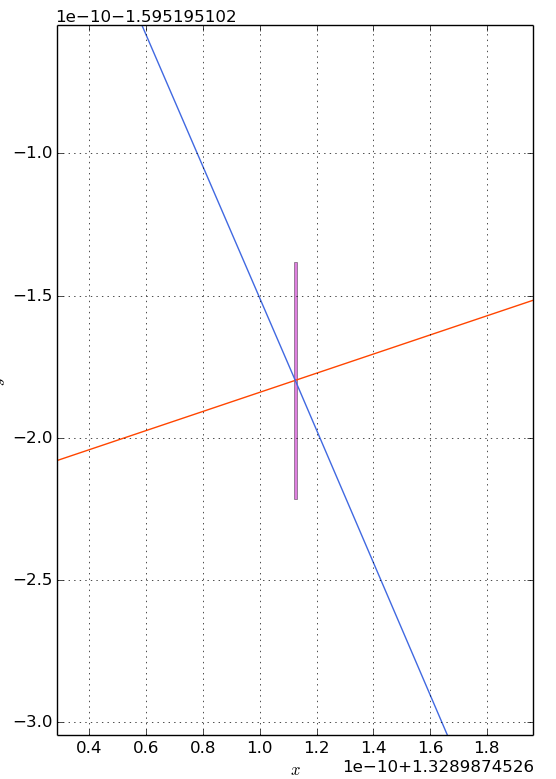
\includegraphics[scale=0.4]{cruce2}
\caption{Cruce de $W^{u},W^{s}$ encontrado con el intervalo b.}
\label{cruce2H}
\end{figure}


\begin{figure}[H]
\centering
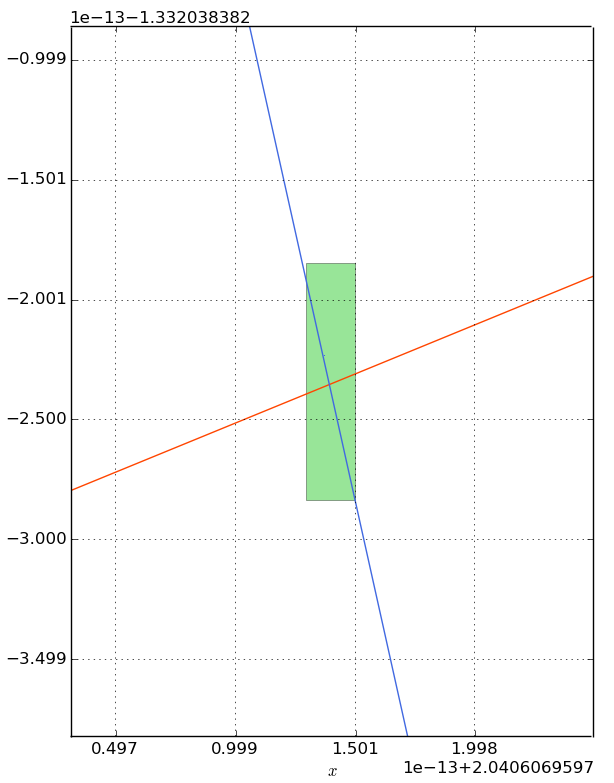
\includegraphics[scale=0.4]{cruce3}
\caption{Cruce de $W^{u},W^{s}$ encontrado con el intervalo c.}
\label{cruce3H}
\end{figure}


\begin{figure}[H]
\centering
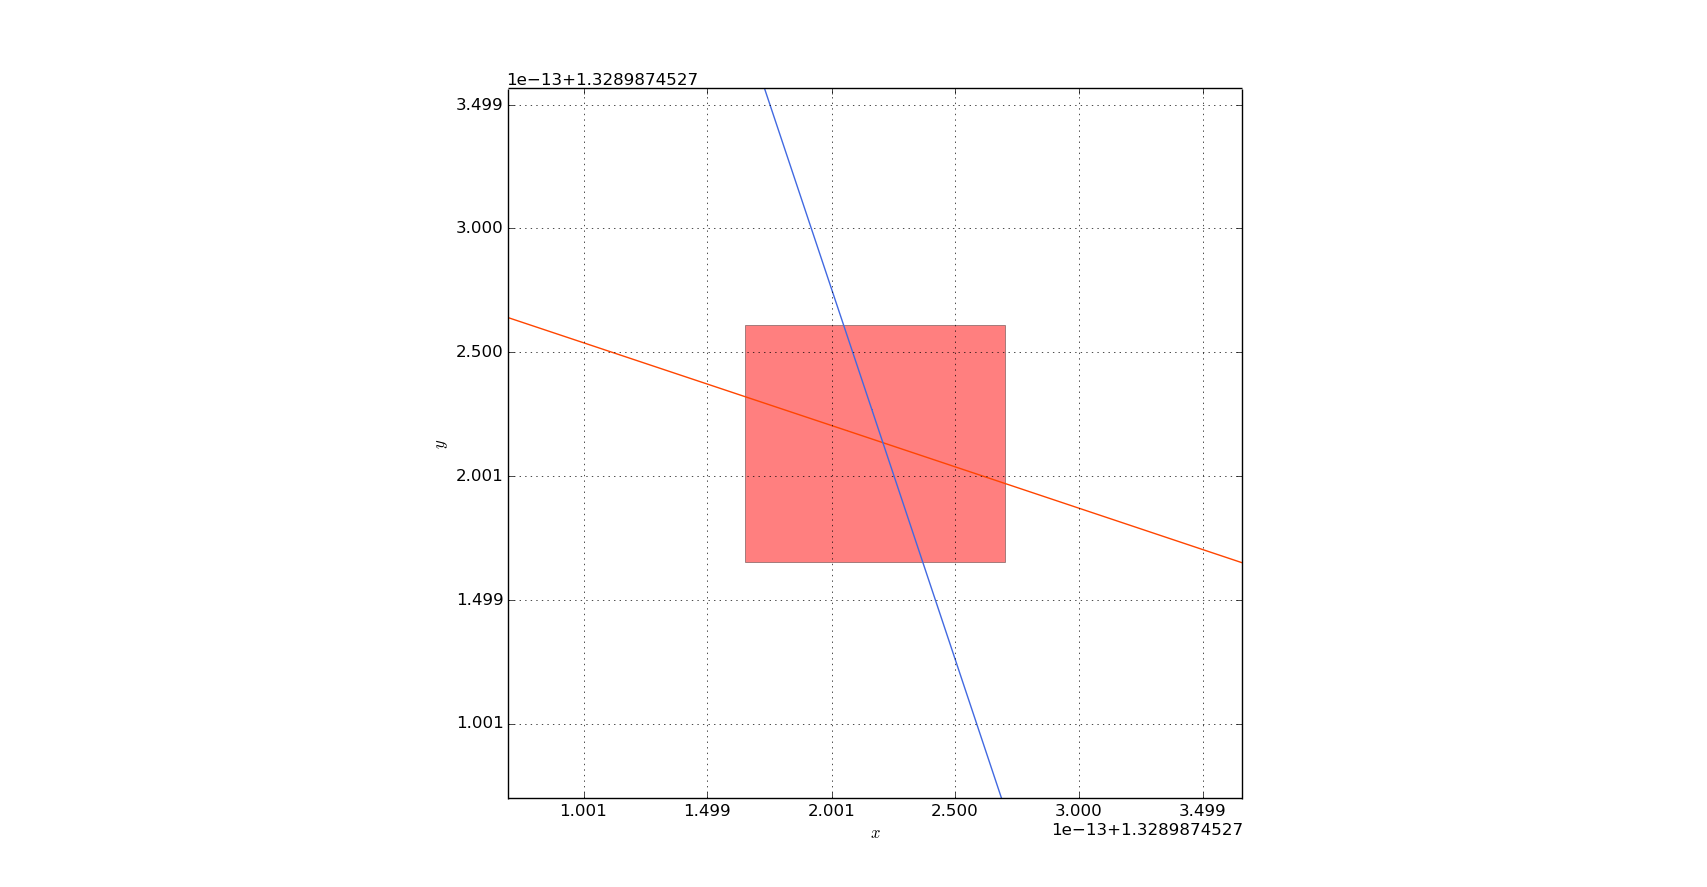
\includegraphics[scale=0.4]{cruce5}
\caption{Cruce de $W^{u},W^{s}$ encontrado con el intervalo e.}
\label{cruce5H}
\end{figure}

\begin{figure}[H]
\centering
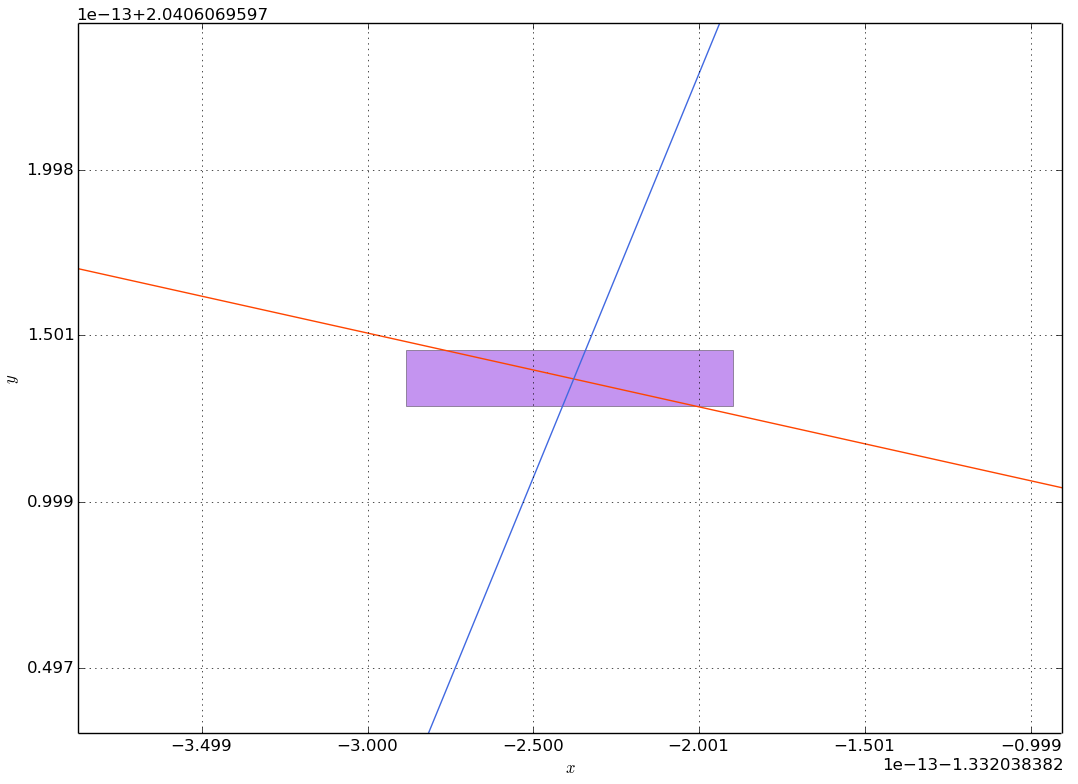
\includegraphics[scale=0.4]{cruce6}
\caption{Cruce de $W^{u},W^{s}$ encontrado con el intervalo f.}
\label{cruce6H}
\end{figure}

\begin{figure}[H]
\centering
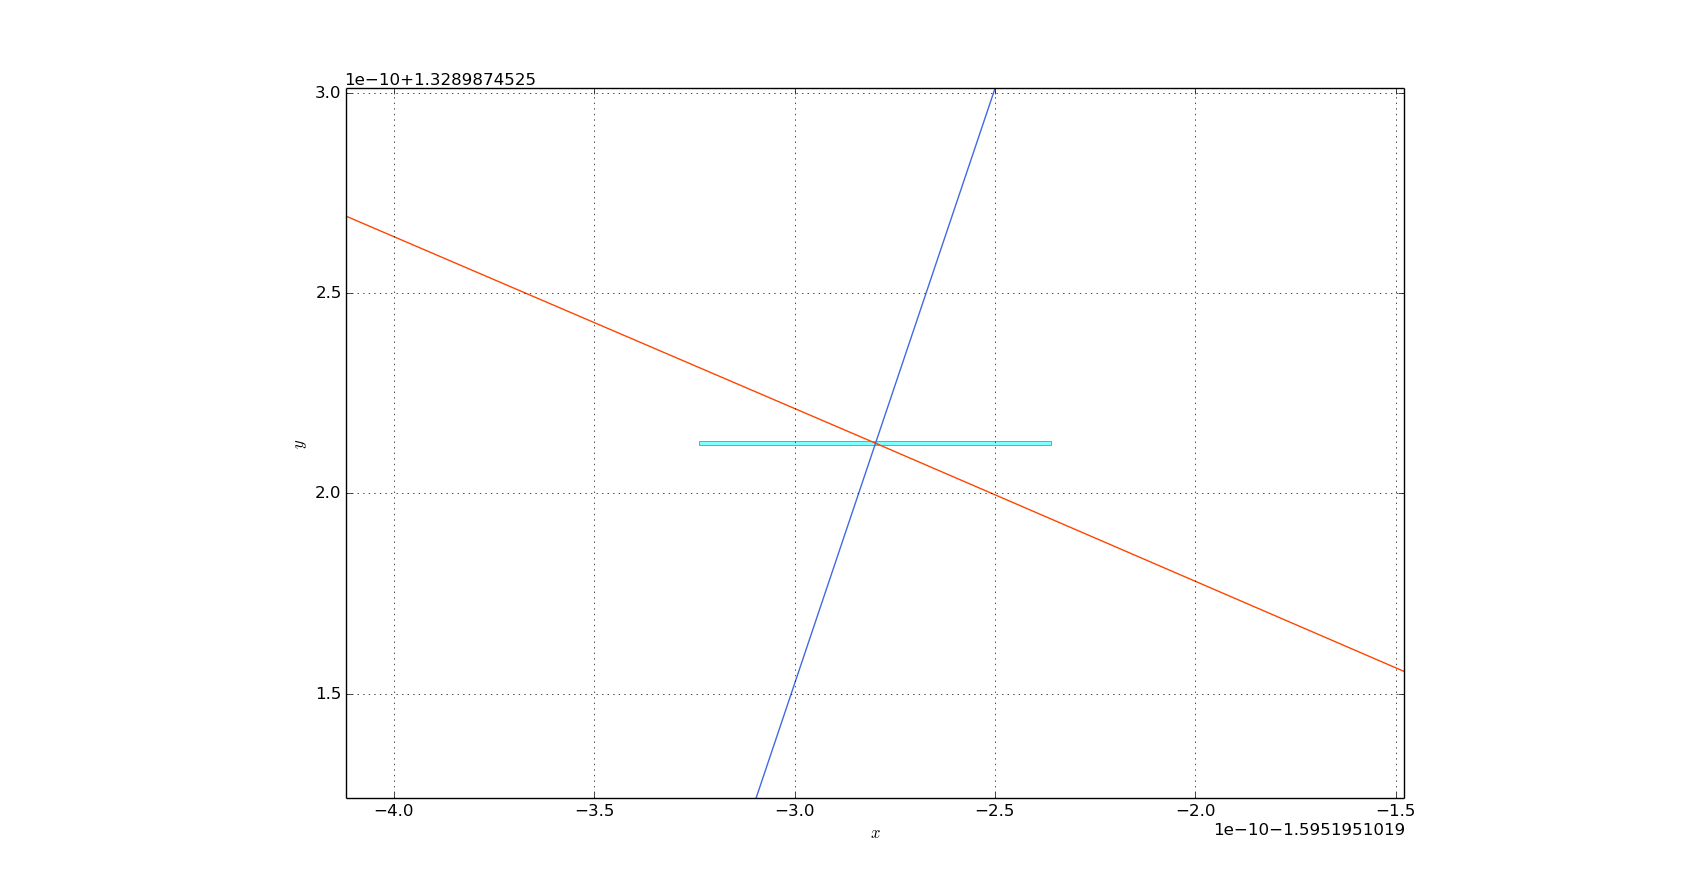
\includegraphics[scale=0.4]{cruce7}
\caption{Cruce de $W^{u},W^{s}$ encontrado con el intervalo g.}
\label{cruce7H}
\end{figure}

\begin{figure}[H]
\centering
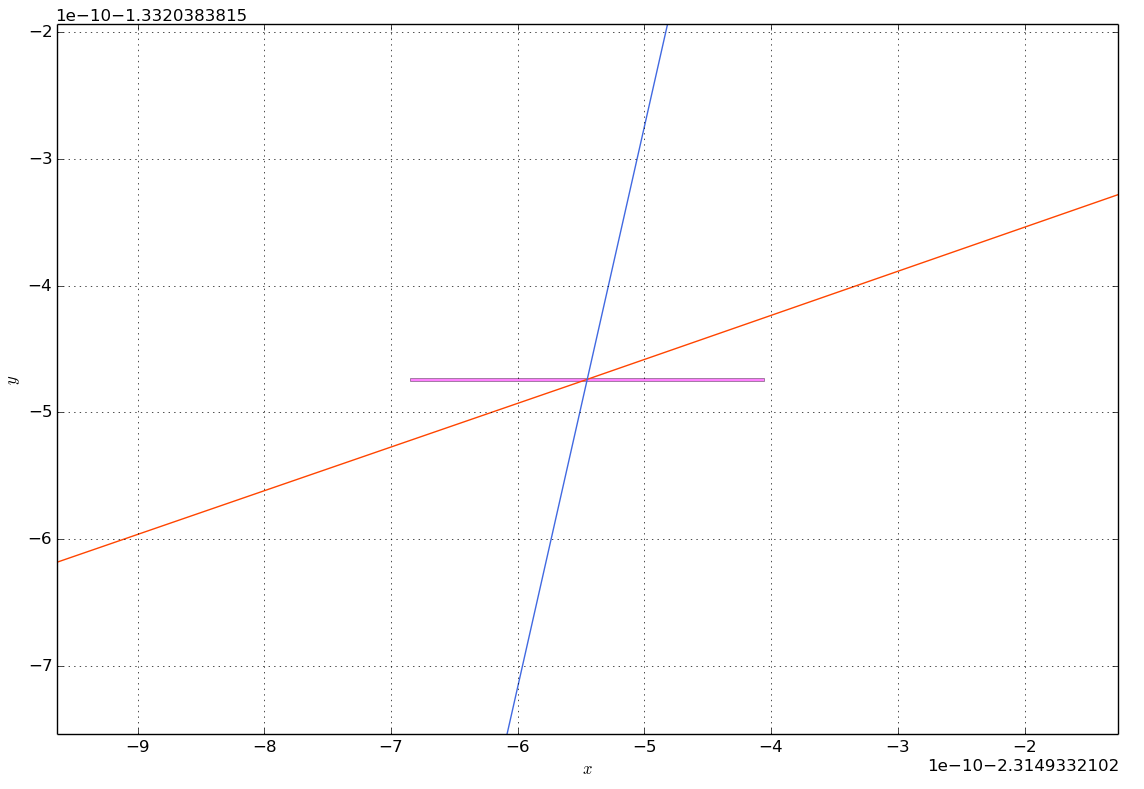
\includegraphics[scale=0.4]{cruce8}
\caption{Cruce de $W^{u},W^{s}$ encontrado con el intervalo h.}
\label{cruce8H}
\end{figure}

La zona rectangular sombreada en cada gráfica representa el producto cartesiano de los intervalos donde se encuentra la solución. Podemos observar que de hecho cada zona contiene el cruce de las variedades garantizando así que en el intervalo propuesto hay un cruce lo cual representa un punto homoclínico. Algunos de los cruces como los de las figuras \ref{cruce1H}, \ref{cruce2H}, \ref{cruce7H} y \ref{cruce8H} son realmente imperceptibles. Este tipo de resultados son útiles para hablar sobre caos topológico \cite{devaney},\cite{gerald}.\\

Para complementar todo este análisis se puede obtener una gráfica de las superficies que forman las variedades al cambiar el parámetro del mapeo lo que nos da una idea de como se ven las superficies y además de como se comportan las intersecciones. La figura \ref{SuperficiesH} muestra las superficies formadas por las variedades para ciertos valores del parámetro $a$. Algunas gráficas más se encuentran en \url{https://github.com/alvarezeve/Tesis-Variedades-Estables-e-inestables/blob/master/Superficies.ipynb}
\begin{figure}[H]
\centering
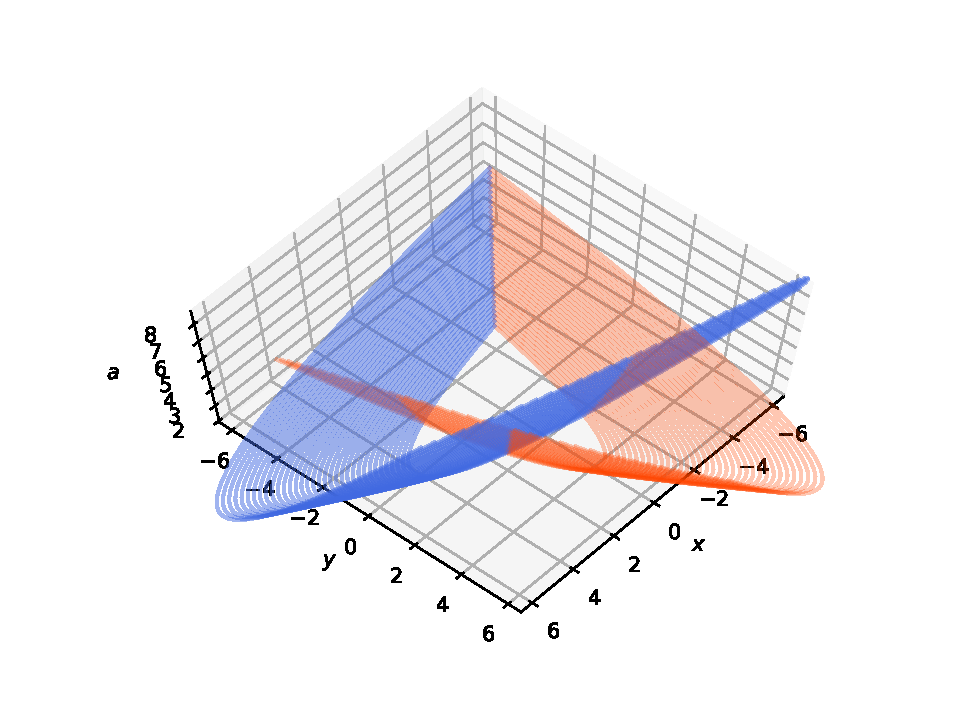
\includegraphics[scale=0.9]{HenonV}
\caption{Superficies en el mapeo de Hénon formadas por las variedades.}
\label{SuperficiesH}
\end{figure}



\subsection{Mapeo exponencial}
Las intersecciones en el caso del mapeo \eqref{Jung} se calcularon usando como en los casos anteriores el mapeo inverso \eqref{jungI}. Este mapeo representa un mayor reto en cuanto al orden del polinomio, pes la presencia de la exponencial hace que la parametrización sea sensible al orden del mismo. Para el siguiente ejemplo se utilizó un polinomio de orden 86 y una tolerancia en el método de Newton de $10-6$ y se calcularon los cruces de las variedades como en los otros casos. Las siguientes fueron las secciones en términos del parámetro $t,\tau$ dónde se encontraron los cortes. 
\begin{itemize}
\item[a)] Root$([-0.985068, -0.985067] \times [5.99488, 5.99489]$, :unique)
\item[b)] Root$([-3.46215, -3.46214] \times [5.49229, 5.4923]$, :unique)
\item[c)] Root$([-3.77896, -3.77895] \times [1.56269, 1.5627]$, :unique)
\end{itemize}
La representación de los cortes se puede ver en la figura \ref{jung_cortes}.
\begin{figure}[H]
\centering
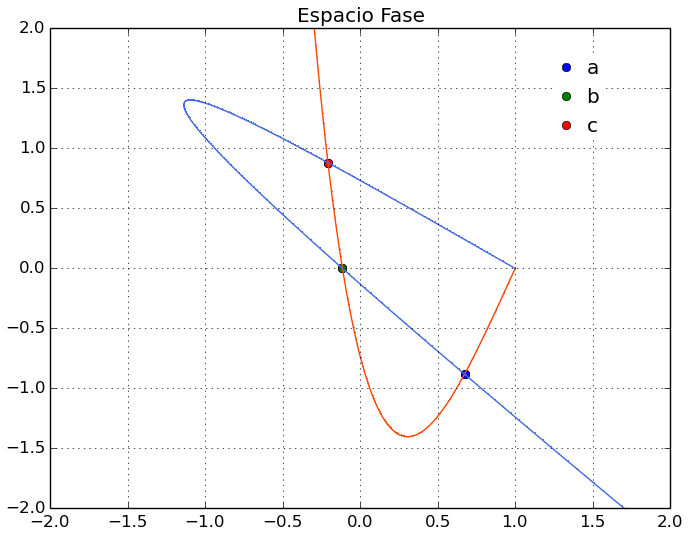
\includegraphics[scale=0.5]{cruces_jung1}
\caption{Intersecciones en el mapeo exponencial con $a=5.7$.}
\label{jung_cortes}
\end{figure}

Tomando los cruces a escala del intervalo se obtuvieron las figuras \ref{jung_corte1}-\ref{jung_corte3}.

\begin{figure}[H]
\centering
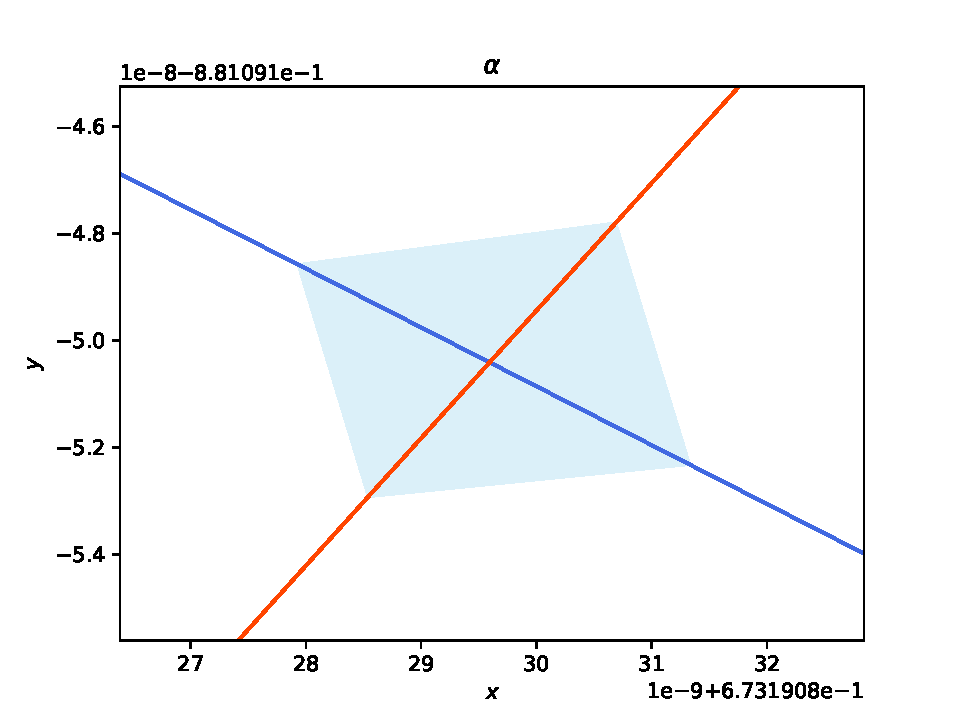
\includegraphics[scale=0.4]{cruce_a}
\caption{Intersección en el intervalo a.}
\label{jung_corte1}
\end{figure}


\begin{figure}[H]
\centering
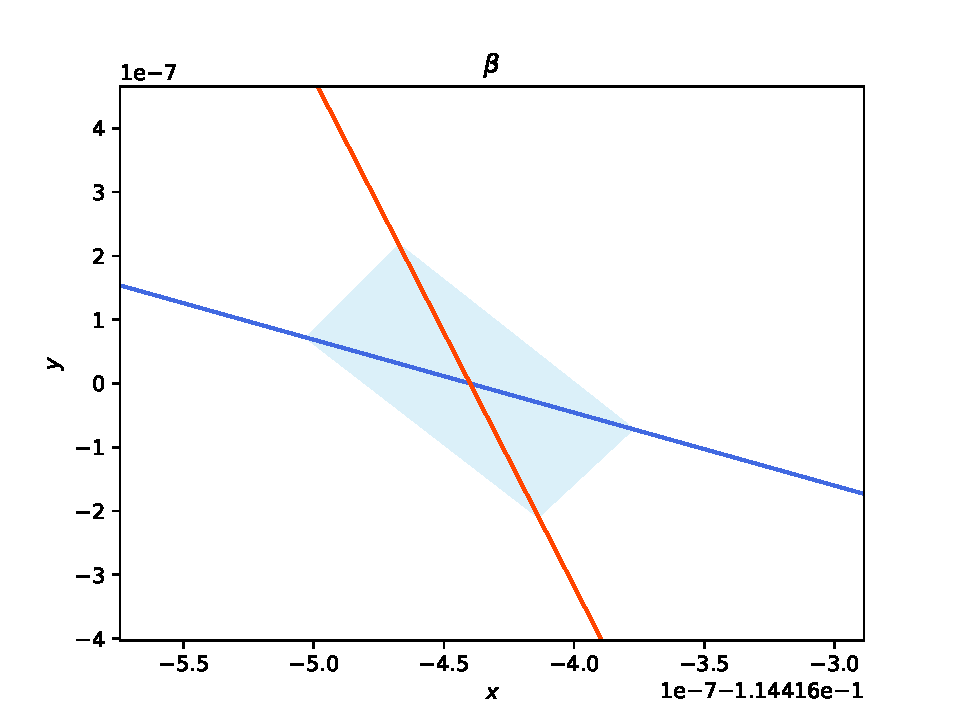
\includegraphics[scale=0.4]{cruce_b}
\caption{Intersección en el intervalo b.}
\label{jung_corte2}
\end{figure}


\begin{figure}[H]
\centering
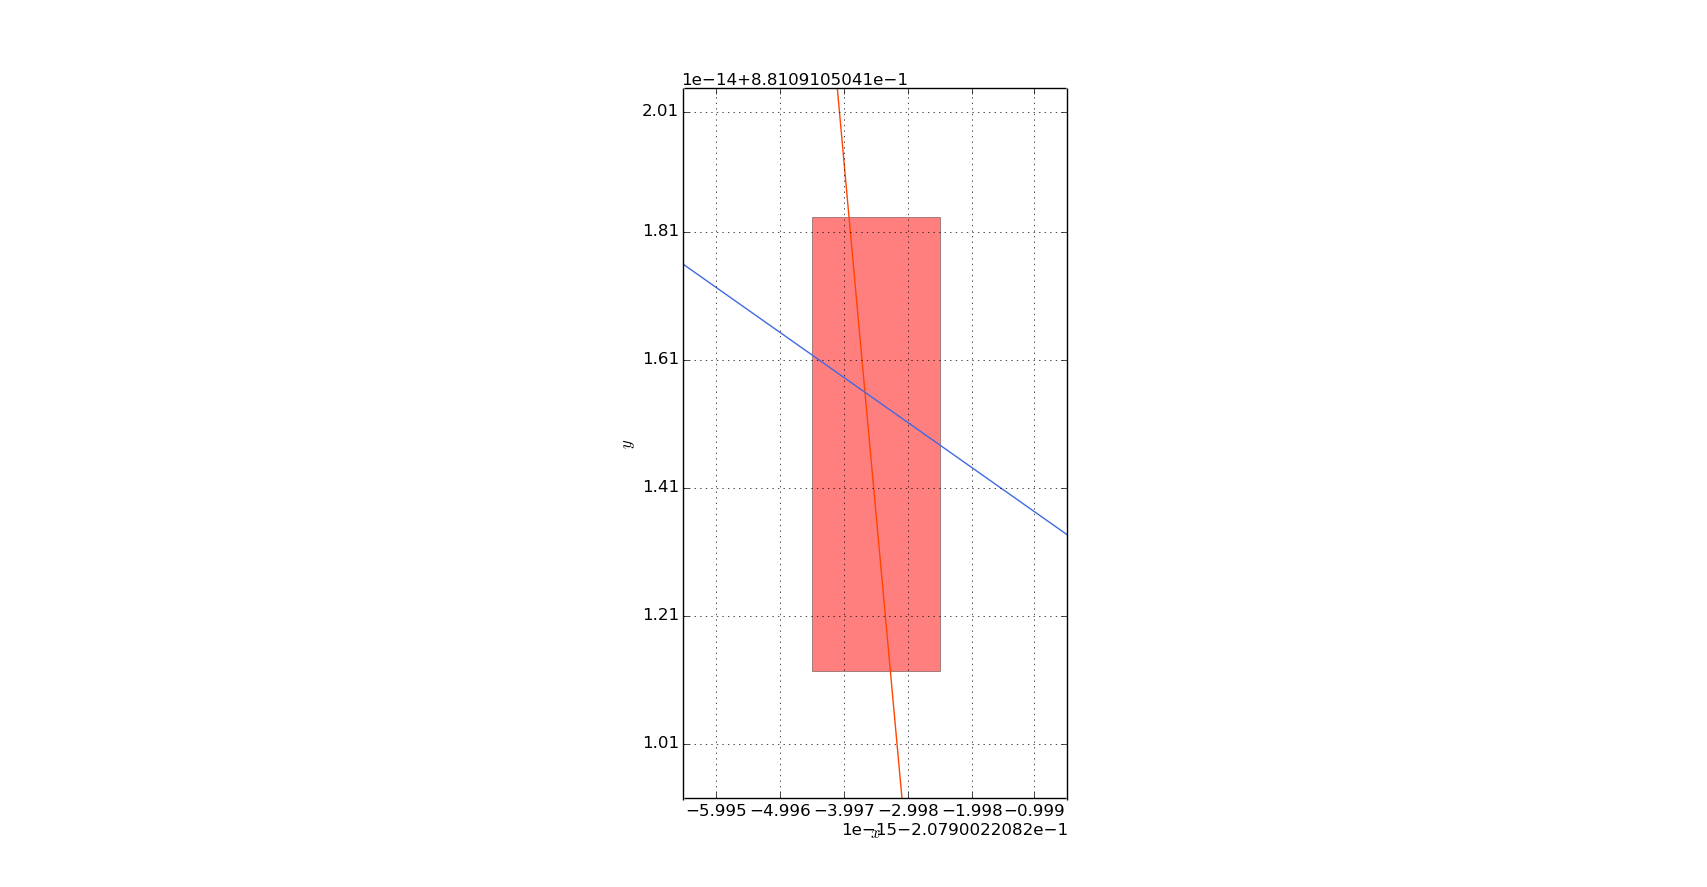
\includegraphics[scale=0.4]{cruce_c}
\caption{Intersección en el intervalo c.}
\label{jung_corte3}
\end{figure}

Las escalas en las que se observan los cortes de las variedades son pequeños comparados con la escala del mapeo, tanto que si se graficaran en el espacio fase no se podrían observar. Como ya se mencionó estos garantiza que existen tres puntos homoclínicos en el intervalo usado. \\


La implementación del método resultó ser eficiente para encontrar los polinomios que representan las variedades estable e inestable asociadas a puntos fijos hiperbólicos de los diferentes mapeos. Se tomaron estos tres mapeos para tener un poco de variedad en la forma de las variedades y también de los puntos fijos, en todos los casos el orden de la parametrización afecta de manera diferente, para el caso del mapeo exponencial resulta ser más sensible. En todos ellos un orden mayor contribuye a llegar más lejos en el valor del parámetro con un error bajo y como consecuencia graficar de mejor manera las variedades. Podemos decir que el error lo manipulamos al mover el orden pero también mostramos que se puede mejorar al usar números de precisión extendida. Una característica que se puede observar es que el error se comporta esencialmente de la misma forma para los tres mapeos, creciendo de manera lenta y luego creciendo rápido a partir de cierto valor. \\


El análisis de la convergencia resulta congruente con lo que se puede observar en el error y en las mismas gráficas de las variedades. La convergencia también ayudó a ver que a partir de cierto orden los coeficientes no hacen un cambio significativo, por lo que no es necesariamente cierto que cada que aumentemos el orden se mejorará la parametrización.\\


El cálculo de puntos homoclínicos resulta una de las aplicaciones de tener las variedades parametrizadas. El método junto con las otras paqueterías de Julia son indispensables para hacer este tipo de cálculos de una manera fácil. A pesar de que la aritmética de intervalos arroja resultados garantizados, no hay que olvidar que nuestros polinomios no son calculados de la misma manera, es decir se debe tener siempre en mente que al rededor de cada variedad hay un error asociado. Aún así las intersecciones pueden ser encontradas controlando bien el error en la parametrización y controlando la tolerancia en el método de Newton.

\label{SeccionRectanguloFundamental}\section{Rectángulo fundamental}
Para los mapeos abiertos como lo son Hénon y el mapeo de la sección anterior \eqref{Jung} se puede tener el conjunto fundamental a partir de los polinomios que se obtienen en el método de parametrización. El conjunto fundamental constituye una parte de las variedades mediante la cual se puede obtener toda la dinámica fuera del mismo, llamado también rectángulo fundamental puesto que forma un polígono de cuatro lados que tiene como vértices el punto fijo hiperbólico y las intersecciones de las variedades, como aristas las secciones de las variedades entre estos puntos. Lo que pasa dentro del área del rectángulo fundamental con las variedades estables e inestables es una ventana a escala de lo que pasa si se extienden las variedades. A partir de esto podemos observar lo que se llaman tentáculos o herraduras en la dinámica del mapeo, en la figura \ref{herradura} se muestra un diagrama de este tipo de comportamiento.

\begin{figure}[H]
\centering
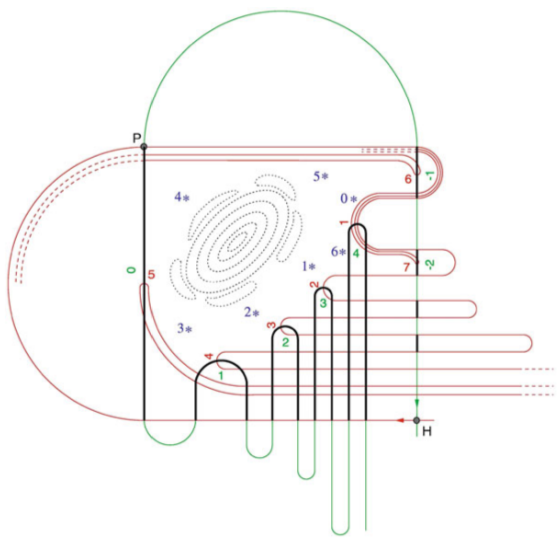
\includegraphics[scale=0.25]{herradura}
\caption{Diagrama ilustrativo de la topología de una herradura en un sistema Hamiltoniano de dos dimensiones, H denota el punto fijo hiperbólico y P la primera intersección. Los tentáculos de la variedad estable son enfatizados con color negro. Tomada de \cite{Ying}, pp.215.}
\label{herradura}
\end{figure}

Una manera de llegar a observar estas estructuras con los polinomios de la parametrización sería usando polinomios de ordenes grandes, pero como hemos visto en la sección \ref{SeccionEstandar} el error no cambia mucho cuando pasamos de cierto grado en el polinomio. Sin embargo si notamos que nuestra parametrización representa, con cierto error, una sección de la variedad estable o inestable, entonces podemos aplicar el mapeo a la parametrización de manera que iteramos, análogamente a iterar puntos. Con esta idea se pudo encontrar parte de las estructuras mostradas en la figura \ref{herradura}, para los mapeos \eqref{Henon}, \eqref{Jung}.


En el caso del mapeo de Hénon con $a=6.5$ se calcularon polinomios de orden 250 usando números de precisión extendida ($W_{0}^{s},W_{0}^{u}$), además calcular la variedad estable usando el mapeo de Hénon inverso \eqref{HenonI}. En este caso se necesitó un valor máximo del parámetro $t=100$ para obtener el rectángulo fundamental, que se muestra en la figura \ref{rectangulo0}, para éstas condiciones el error es menor a $10^{-73}$.

\begin{figure}[H]
\centering
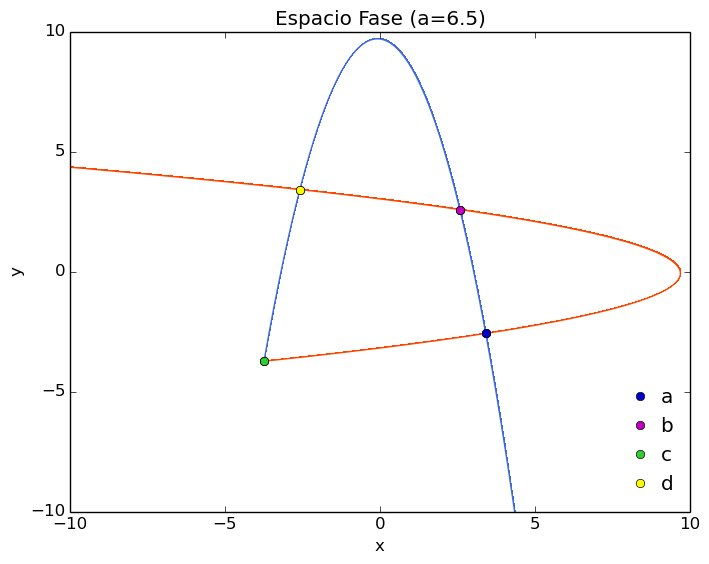
\includegraphics[scale=0.4]{rectangulo-fundamental}
\caption{Variedades estable e inestable de orden 250, para el mapeo de Hénon con $a=6.5,b=1.$, con $t_{max}=100$. El punto c) denota el punto fijo mientras que  a),b),d) son las primeras intersecciones de las variedades.}
\label{rectangulo0}
\end{figure}

\begin{figure}[H]
\centering
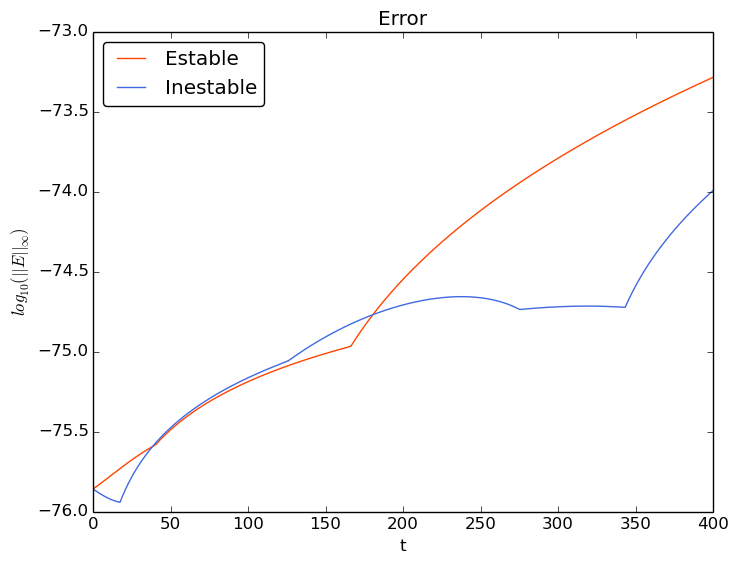
\includegraphics[scale=0.6]{error-rectangulo}
\caption{Error asociado al cálculo de las variedades en la figura \ref{rectangulo0}}.
\label{ErrorRectangulo0}
\end{figure} 

Reescribiendo la ecuación de invariancia \eqref{Ecua de invariancia} para el caso de la variedad estable, tenemos que:
\begin{eqnarray}
f_{a,b}^{-1}(W_{0}^{s}(t))=W_{0}^{s}(\lambda^{s}t).
\label{InvarianciaEstable1}
\end{eqnarray}
%\begin{eqnarray}
%f_{a,b}(W_{0}^{u}(t))=W_{0}^{u}(\lambda^{u}t)
%\label{InvarianciaInestable1}
%\end{eqnarray}
Si aplicamos el mapeo de Hénon inverso \eqref{HenonI} a la ecuación \eqref{InvarianciaEstable1} resulta
\begin{eqnarray}
W_{0}^{s}(t)=f_{a,b}(W_{0}^{s}(\lambda^{s}t)),
\label{InvarianciaEstable2}
\end{eqnarray}

%\begin{eqnarray}
%W_{0}^{u}(t)=f_{a,b}^{-1}(W_{0}^{u}(\lambda^{u}t))
%\label{InvarianciaInestable2}
%\end{eqnarray}
como el parámetro es una variable muda podemos reescribir \eqref{InvarianciaEstable2}, 
\begin{eqnarray}
W_{0}^{s}(\frac{t}{\lambda^{s}})=f_{a,b}(W_{0}^{s}(t)).
\label{InvarianciaEstable3}
\end{eqnarray}

%\begin{eqnarray}
%W_{0}^{u}(\frac{t}{\lambda^{u}})=f_{a,b}^{-1}(W_{0}^{u}(t)).
%\label{InvarianciaInestable3}
%\end{eqnarray}
Siendo que $\vert \lambda^{s} \vert < 1 $ la ecuación \eqref{InvarianciaEstable3} muestra que aplicar el mapeo es análogo a tener la variedad estable evaluada en un valor mayor del parámetro, puesto que $1/\lambda^{s}>1$. Este resultado es análogo para la variedad inestable. Usando esto se obtuvo la figura \ref{Rectangulo1}, que muestra el resultado de la iterar una vez, $(W_{x1}^{s},W_{y1}^{s})=f_{a,b}(W_{x}^{s},W_{y}^{s})$, análogamente para las inestables, evaluando los nuevos polinomios exactamente en los mismos intervalos que en el caso de la figura \ref{rectangulo0}.
\begin{figure}[H]
\centering
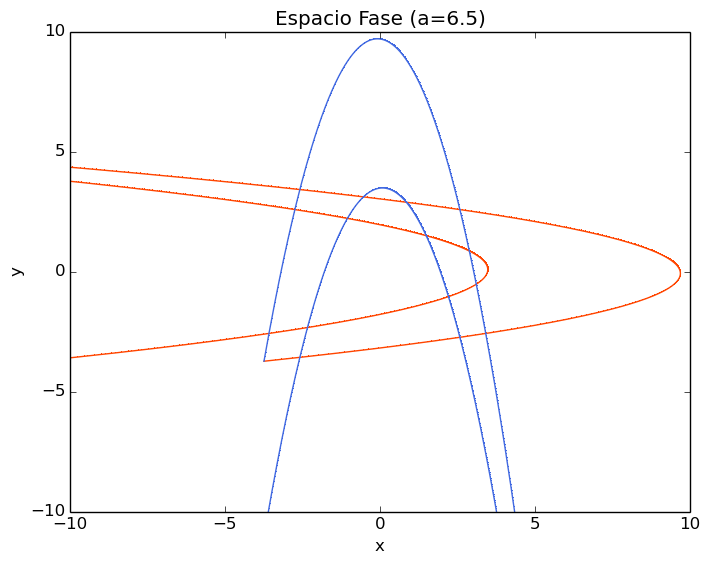
\includegraphics[scale=0.5]{rectangulo1}
\caption{Primera aplicación del mapeo a los polinomios de orden 250, $t_{max}=100$}.
\label{Rectangulo1}
\end{figure}
El cálculo con el que se obtiene la figura \ref{Rectangulo1} produce un nuevo polinomio el cual tiene asociado también un error numérico. Para saber cuál es este error se usó la ecuación \eqref{InvarianciaEstable3},
\begin{eqnarray}
E_{1}(t)=\parallel W_{0}^{s}(\frac{t}{\lambda^{s}})-f_{a,b}(W_{0}^{s}(t))\parallel_{\infty},
\label{error-1aplicacion}
\end{eqnarray}
está forma es análoga a la ecuación \eqref{Ecua de invariancia resta} la cual se representa en la figura \ref{error-1iteracion}. De la misma manera se evalúa el error en las aplicaciones consecutivas, el cual podemos expresar como
\begin{eqnarray}
E_{n}(t)=\parallel (f^{-1}_{k})^{n}(W_{0}^{s}(\frac{t}{\lambda^{s}}))- (f^{-1}_{k})^{n-1}(W_{0}^{s}(t)))\parallel_{\infty}.
\label{error-n-aplicacion}
\end{eqnarray}
En la ecuación \eqref{error-n-aplicacion} $n$ representa el número de aplicaciones del mapeo mientras que $W_{0}$ es la parametrización inicial calculada mediante el método.

\begin{figure}[h]
\centering
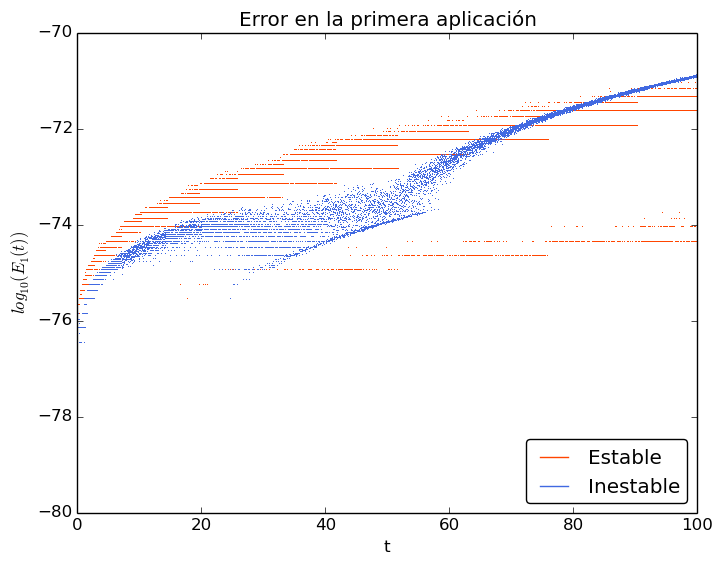
\includegraphics[scale=0.4]{error1ite}
\caption{Error en el polinomio que resulta de aplicar el mapeo a la parametrización de orden 250.}
\label{error-1iteracion}
\end{figure}
Se puede observar en la figura \ref{error-1iteracion} que el error es mínimo en ambas variedades, manteniéndose por debajo del orden de $10^{-70}$, las líneas verticales son producto de valores numéricos que aparecen como cero al evaluar el polinomio a los cuales se les sumó un valor del orden de $10^{-120}$ para poder evaluar el logaritmo base $10$ del error. Si revisamos en la sección \ref{henon-seccion} el error crece mucho más rápido cuando sólo se usa el polinomio que resulta de la parametrización, además de que no es posible llegar tan lejos como se muestra en las figuras \ref{Rectangulo1}-\ref{Rectangulo5}.

La segunda aplicación del mapeo a los polinomios, $(W_{x2}^{s},W_{y2}^{s})=f_{a,b}(W_{x1}^{s},W_{y1}^{s})$ se muestra en la figura \ref{Rectangulo2}, de nuevo usando el mismo valor máximo del parámetro $t$, además en la figura \ref{error-2iteracion} muestra el error asociado a tal resulado.
\begin{figure}[H]
\centering
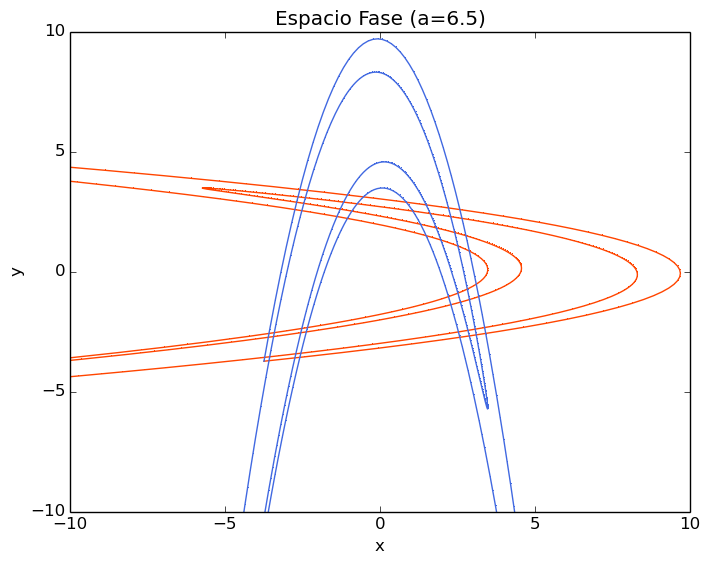
\includegraphics[scale=0.5]{rectangulo2}
\caption{Segunda aplicación del mapeo a los polinomios de orden 250.}
\label{Rectangulo2}
\end{figure}

\begin{figure}[H]
\centering
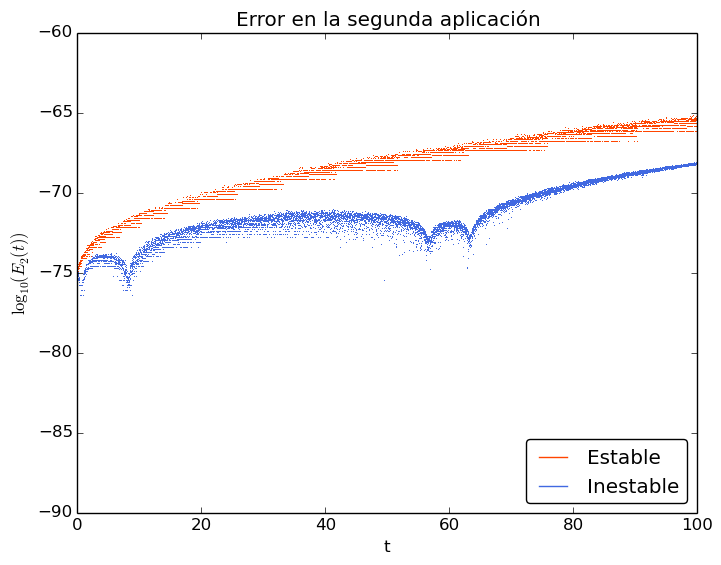
\includegraphics[scale=0.4]{error2ite}
\caption{Error en el polinomio que resulta de aplicar el mapeo por segunda vez a la parametrización de orden 250.}
\label{error-2iteracion}
\end{figure}

De manera sucesiva se aplicaron los mapeos correspondientes hasta iterar cinco veces, siempre conservando el mismo valor máximo del parámetro $t$.
\begin{figure}[H]
\centering
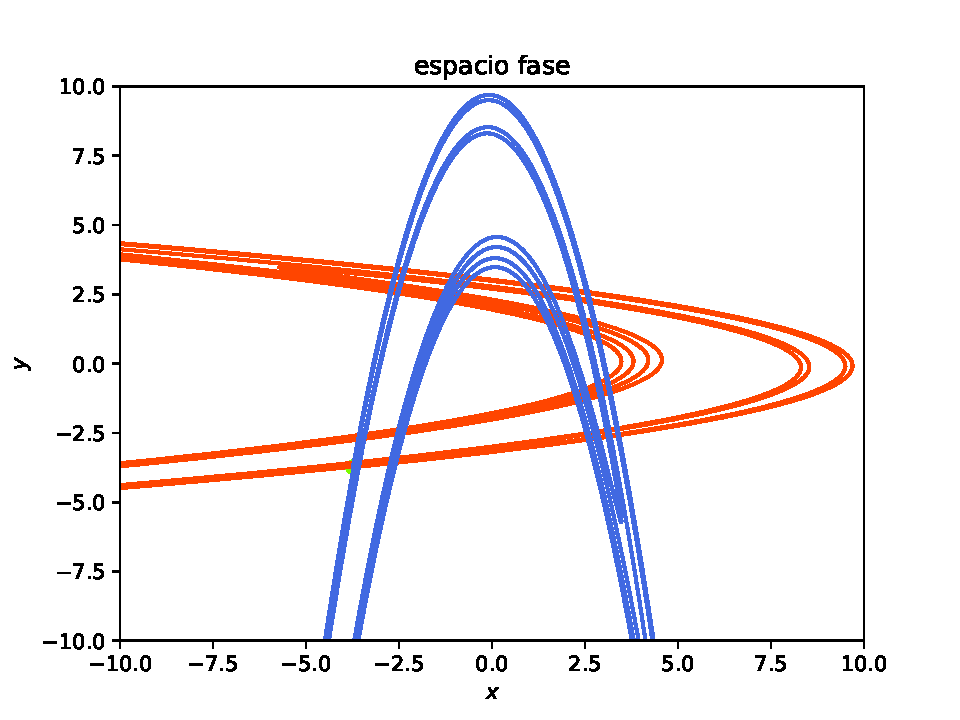
\includegraphics[scale=0.5]{rectangulo3}
\caption{Tercer aplicación del mapeo a los polinomios de orden 250.}.
\label{Rectangulo3}
\end{figure}

\begin{figure}[H]
\centering
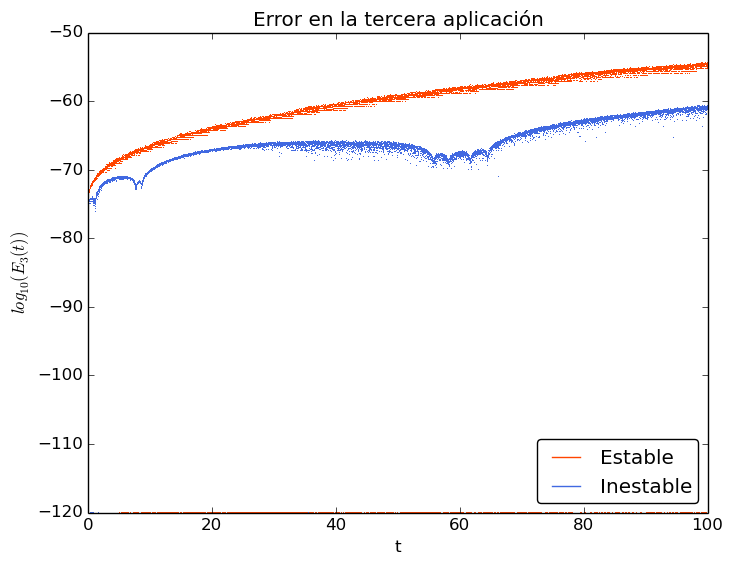
\includegraphics[scale=0.4]{error3ite}
\caption{Error en el polinomio que resulta de aplicar el mapeo por tercera vez a la parametrización de orden 250.}
\label{error-3iteracion}
\end{figure}

\begin{figure}[H]
\centering
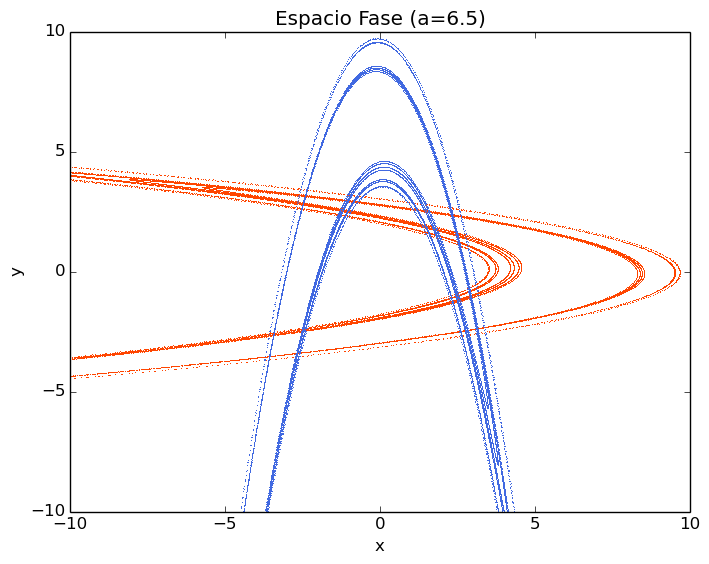
\includegraphics[scale=0.5]{rectangulo4A}
\caption{Cuarta aplicación del mapeo a los polinomios de orden 250.}.
\label{Rectangulo4}
\end{figure}

\begin{figure}[H]
\centering
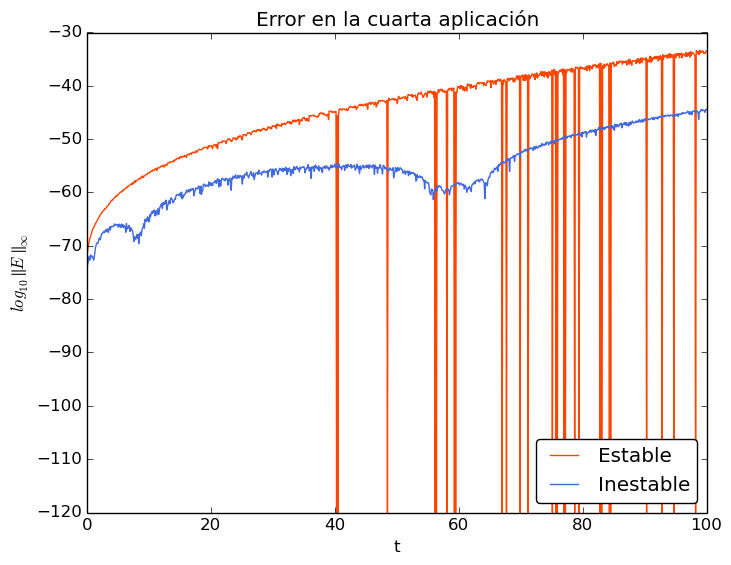
\includegraphics[scale=0.4]{error4ite}
\caption{Error en el polinomio que resulta de aplicar el mapeo por cuarta vez a la parametrización de orden 250.}
\label{error-4iteracion}
\end{figure}

\begin{figure}[H]
\centering
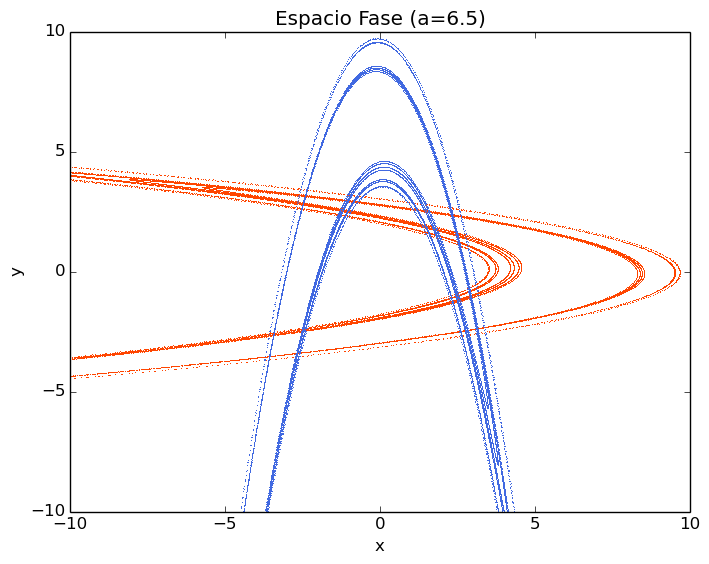
\includegraphics[scale=0.5]{rectangulo5}
\caption{Quinta aplicación del mapeo a los polinomios de orden 250.}.
\label{Rectangulo5}
\end{figure}

\begin{figure}[H]
\centering
\includegraphics[scale=0.4]{error5ite}
\caption{Error en el polinomio que resulta de aplicar el mapeo por quinta vez a la parametrización de orden 250.}
\label{error-5iteracion}
\end{figure}

En las primeras dos aplicaciones del mapeo, \ref{Rectangulo2} y \ref{Rectangulo3}, se puede observar un tentáculo más en cada variedad, mientras que en las siguientes aparecen hasta dos más. La profundidad de tentáculos y la forma en la que se cruzan, depende del valor del parámetro $a$. Hay que enfatizar que para lograr observar estos cruces de manera directa, se debería llegar a valores del parámetro muy grandes comparados con el valor que se usó en todos los casos, lo cual no siempre es posible pues como se vio en la sección \ref{SeccionEstandar} después de cierto orden el error se estanca y no es posible llegar tan lejos con errores controlables, mientras que como muestran las figuras \ref{error-1iteracion}-\ref{error-4iteracion} el error es mucho menor que si se usará un polinomio de orden grande$(>250)$. Con esto mostramos que sólo se necesita conocer el rectángulo fundamental para conocer mucho de la dinámica de las variedades, y por tanto de los cruces entre ellas. 


